%
% common information to the web version and book version
%
% images will be imported by searching the paths set with \graphicspath
% the book.tex or web.tex sets this so the correct resolution images end
% up in the correct document.
% 
% cover is done elsewhere, as this is usually broken out from the 
% ``text block'' for POD publishing--see book.tex
%

\vspace*{5in}
{\large Copyright (C) 2009 Lu Tao  All Rights Reserved.}

This book may not be reproduced in any form without written permission
of the author. 

{\tt 1417274896@qq.com}
\newpage

\vspace*{2in}
\begin{center}
{\LARGE For You}

{\large For auld lang syne}

\vspace*{0.5in}

\includegraphics[width=2in]{me.jpg}
\end{center}
\newpage

\vspace*{1in}
{\LARGE About this book}

This boy is from the steppe.
I've speed most of my childhood in Hohhot, Inner Mongolia. 
The scene of the steppe in my hometown keeps flashing back in my mind these days.  
And it inspires me to make this album in memory of my past days.
These photographs represent some part of me. 
To some extent, to read this book is to read about this boy.

\vspace*{0.25in}

{\LARGE This boy is from the steppe.}

Recently our family (OK, well, I) got the idea to get some chickens and
raise them in the yard. It's fairly common here on the Big Island of
Hawaii, which is mostly still a rural, tropical, agricultural kind of
place. We live on the edge of the largest town on the island, Hilo, with
a population of roughly around 40 thousand (40759 in the 2000 census).

Chickens, dogs, wild pigs and cattle can be heard in our neighborhood,
so I wasn't worried that my chickens would disturb anyone. Especially
since I had no intention of getting a rooster. I thought it would be a
fun project for the kids, and maybe we'd get some fresh eggs every week,
to boot. 

Although we have owned other kinds of critters through the years we had
never had chickens before, so this project was definitely one of
discovery. 
Thankfully, with sites like {\tt mypetchicken.com} and 
{\tt backyardchickens.com} to
guide us, as well as plenty of advice from friends and co-workers with
chickens, we're well on our way. This then, is the practical story of
how we went about it for the first month. Because you see, Solo Photo
Book Month doesn't wait for the full story of the chickens; there is
only time for the beginning of the story--all the photos have to be taken
in a 30 day period of time, and a book must be produced at the end.

And so, without further ado, 

{\Large {\em BacGawwwwk!!}}
\newpage

\vspace*{3in}
\begin{center}
\Huge{This boy is from the steppe.}
\end{center}
\newpage

\pagestyle{plain}

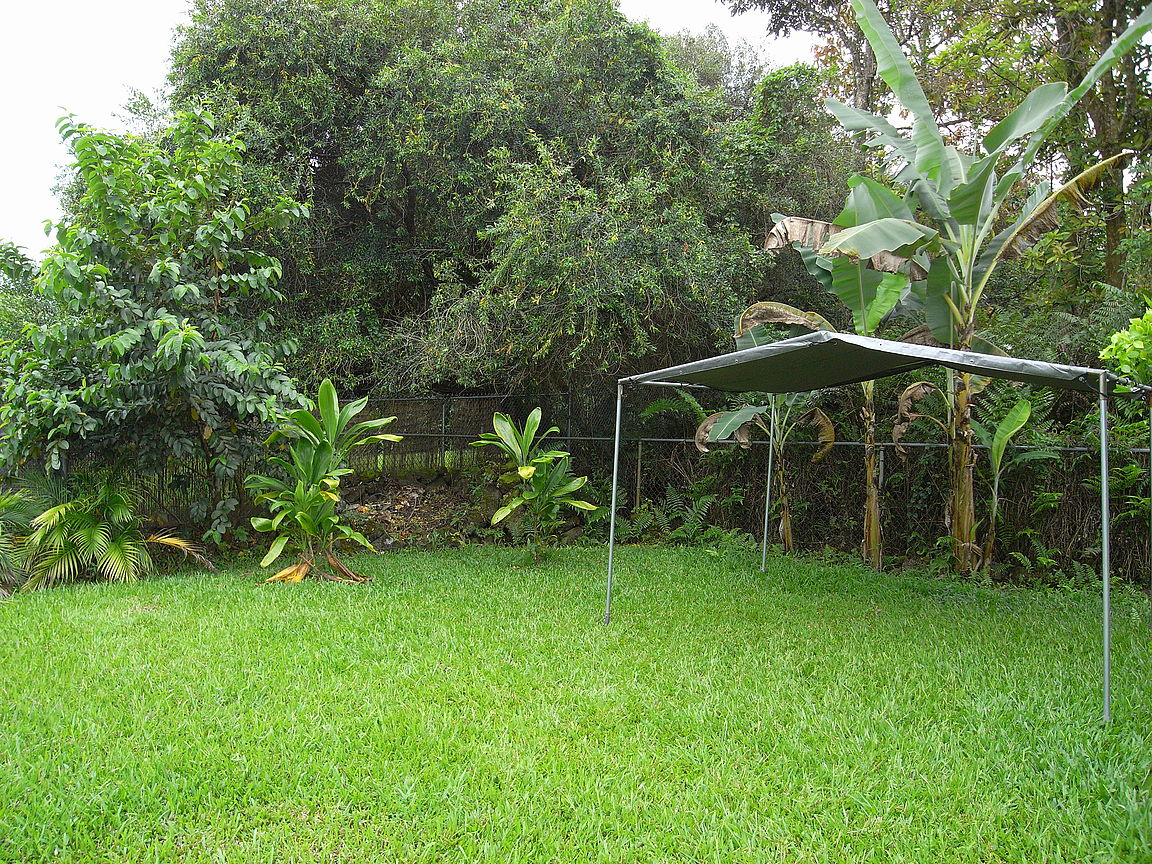
\includegraphics[width=8in]{R20090523-142346}

Before we brought anything home, I thought it might be a good idea to
figure out the where and how of a coop. It rains a fair bit here so I
knew I'd need some kind of cover for the chickens. I wasn't ready to
build anything lavish until I'd figured out a few more things about what
the chicken's needs would be. I did have this little tarp around, the
kind that are ubiquitous around here for temporary permanent roofs. Next
to the bananas in the corner of the yard seemed like a good spot, close
to the compost pile and well away from the house. 
\newpage

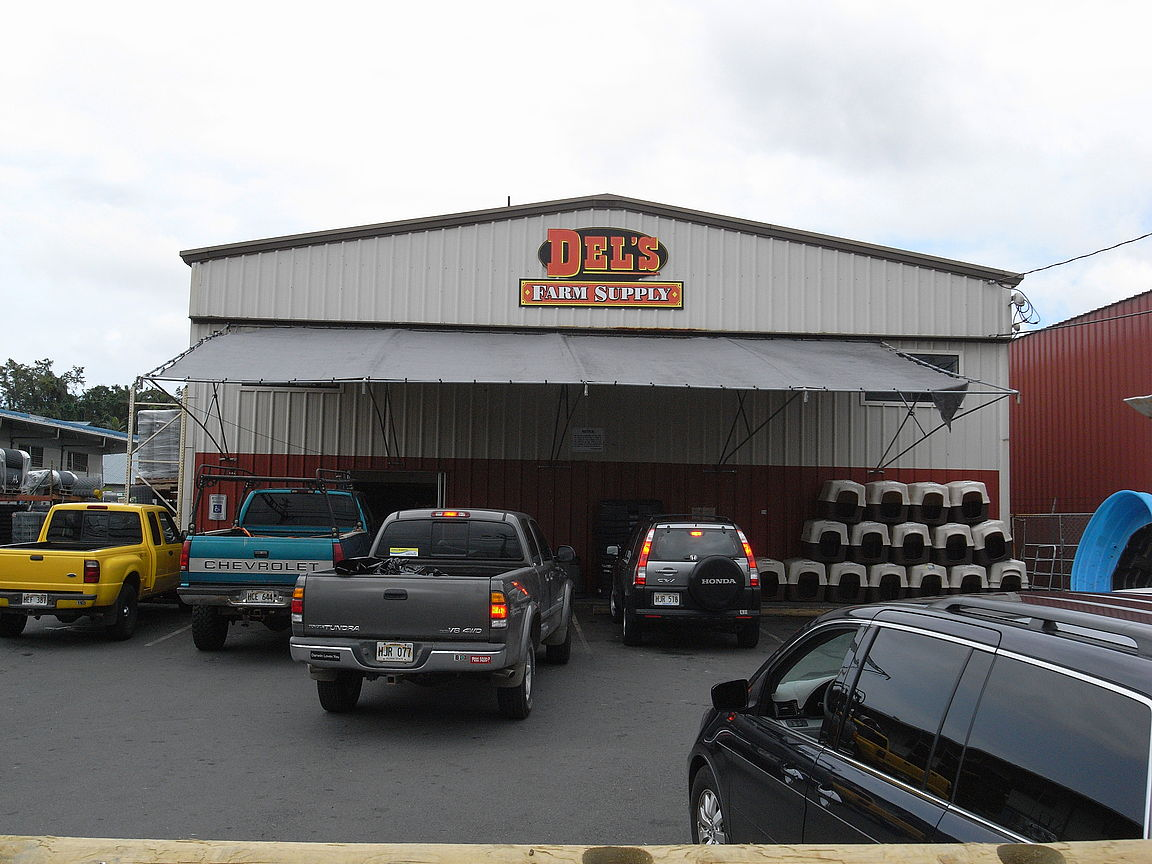
\includegraphics[width=8in]{R20090523-144104}

On a late day in May we headed into town to Del's to pick up the chicks,
as well as any supplies we would need.  Del's had told me earlier they'd
have chicks stocked until June. 
\newpage

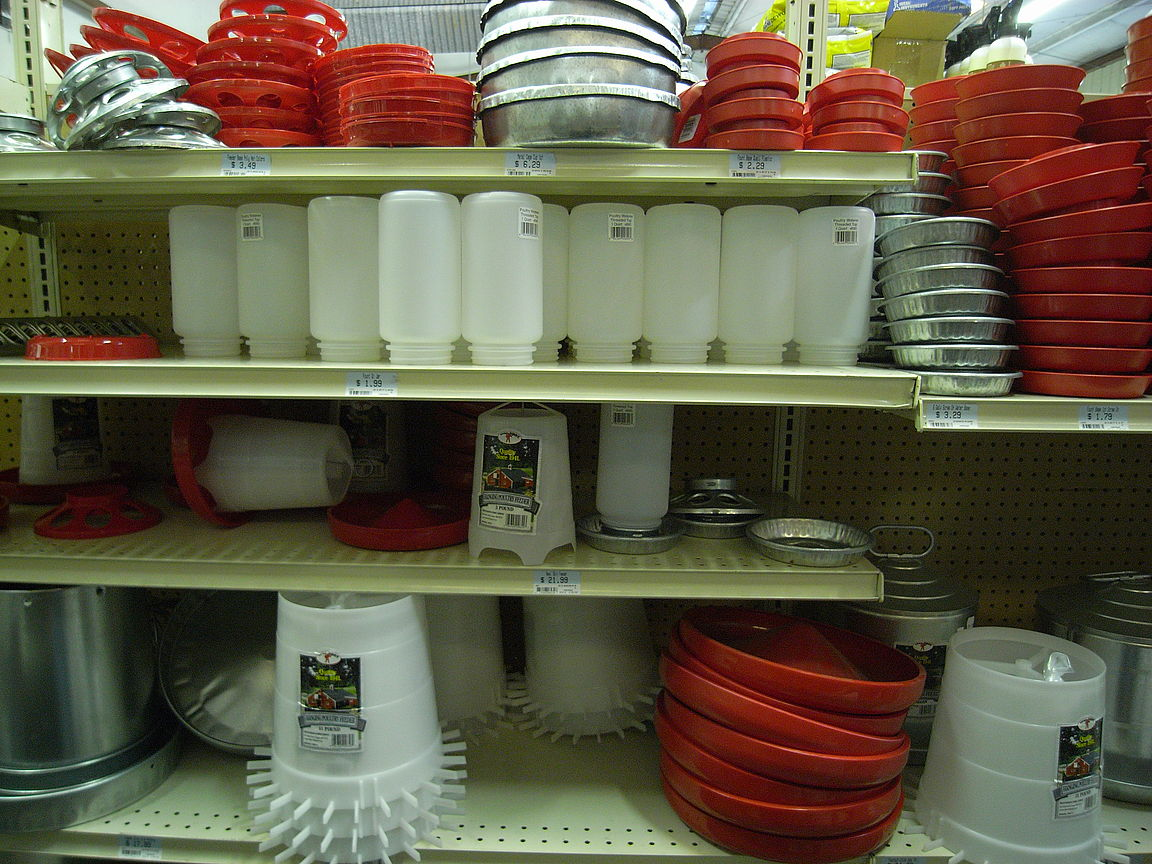
\includegraphics[width=8in]{R20090523-145237}

First stop, supplies.  There was a large selection to choose from.  I
made a couple of reasonable guesses based on what I'd seen in the chick
tub up at the front of the store, and picked up a waterer, a feeder and
a lamp to keep the chicks warm. 
\newpage

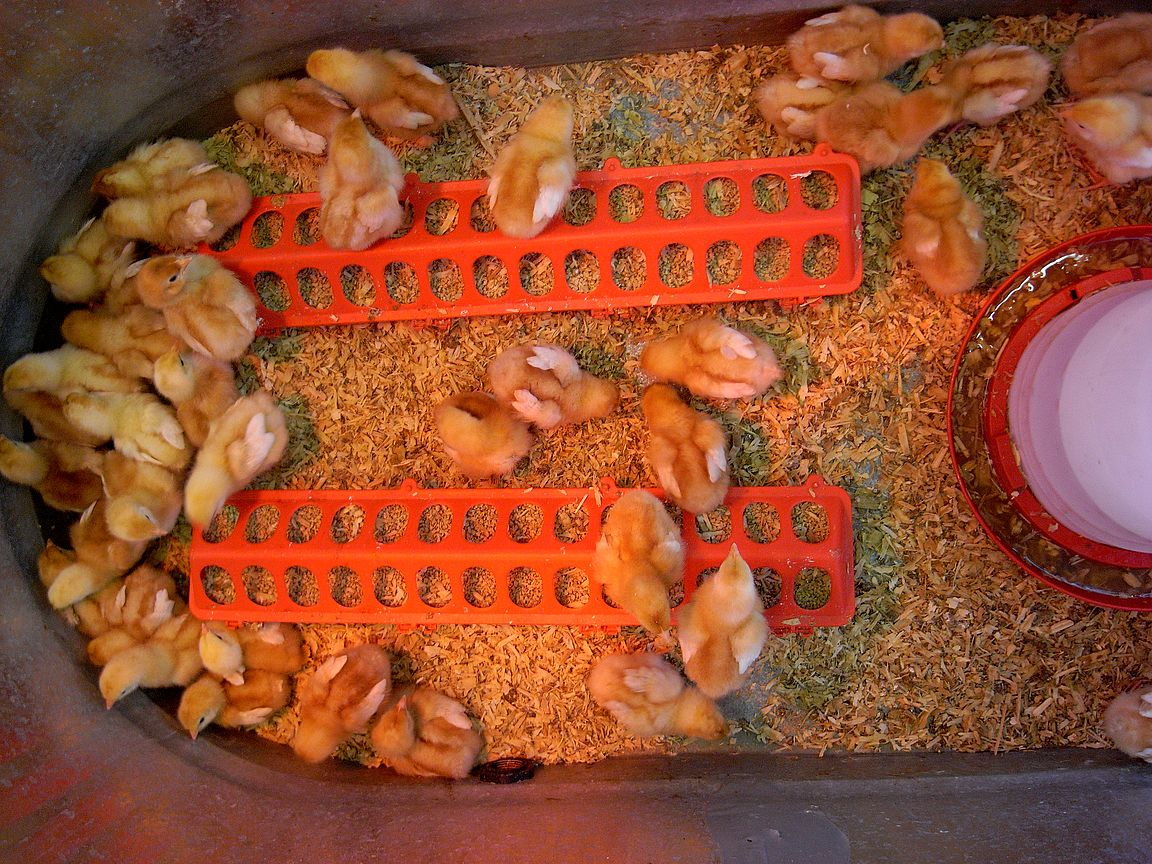
\includegraphics[width=8in]{R20090523-144552-levels}

Next up, the chicks.  They had plenty of Rhode Island Reds on hand, but
the clerk told me they were out of chick feed, and she advised me not to
pick up any chicks unless I had feed.  I called around to the couple of
other farm stores in town, but they were closed.  The kids and I were
pretty disappointed, but the clerk assured me they'd have some feed
coming in next week, so we paid for the supplies and left without any
chicks. 
\newpage

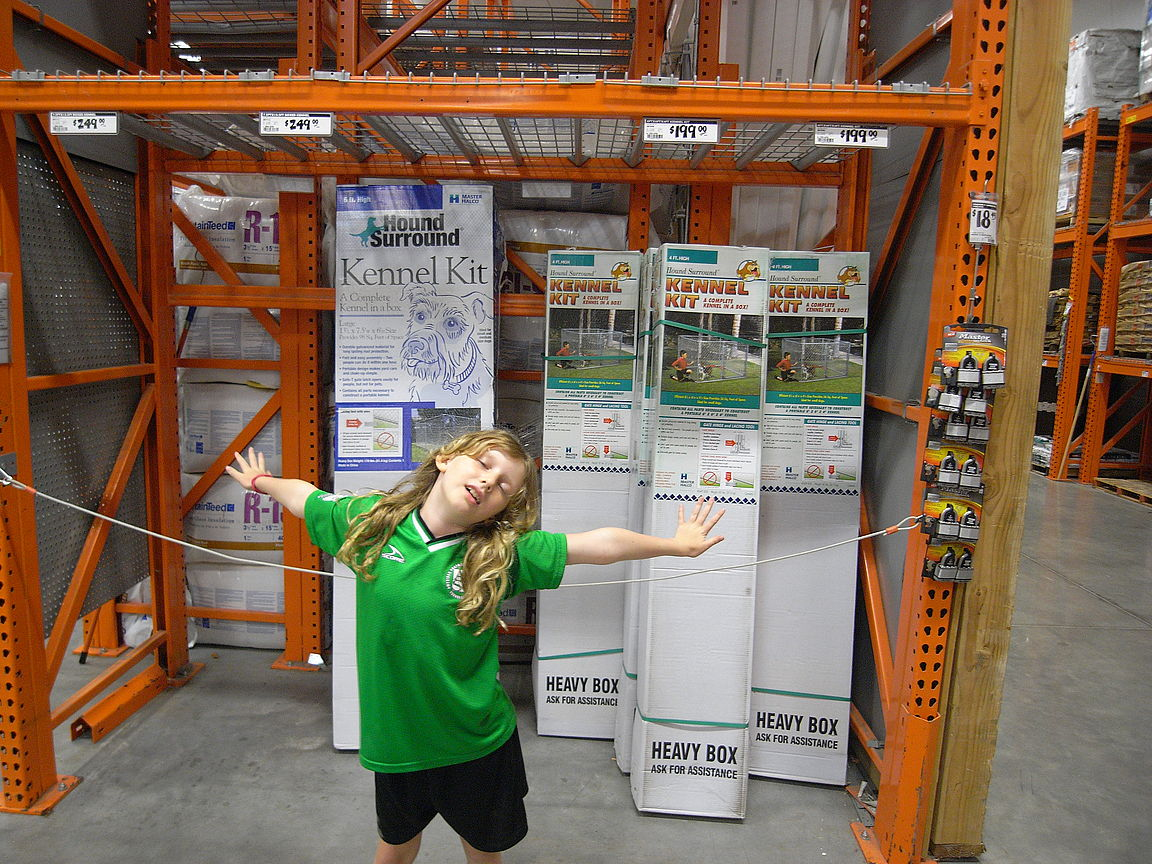
\includegraphics[width=8in]{R20090523-153735}

Next stop was Home Despot, er, Depot.  I had the beginnings of a plan in
mind for a chicken coop.  My idea was to use a dog kennel as a starter
coop.  HD had some inexpensive dog kennel kits, and I knew that with the
galvanized steel I'd have something that could stand up to the rain, sun
and termites.  I needed something to keep the chickens in, and predators
out. 
\newpage

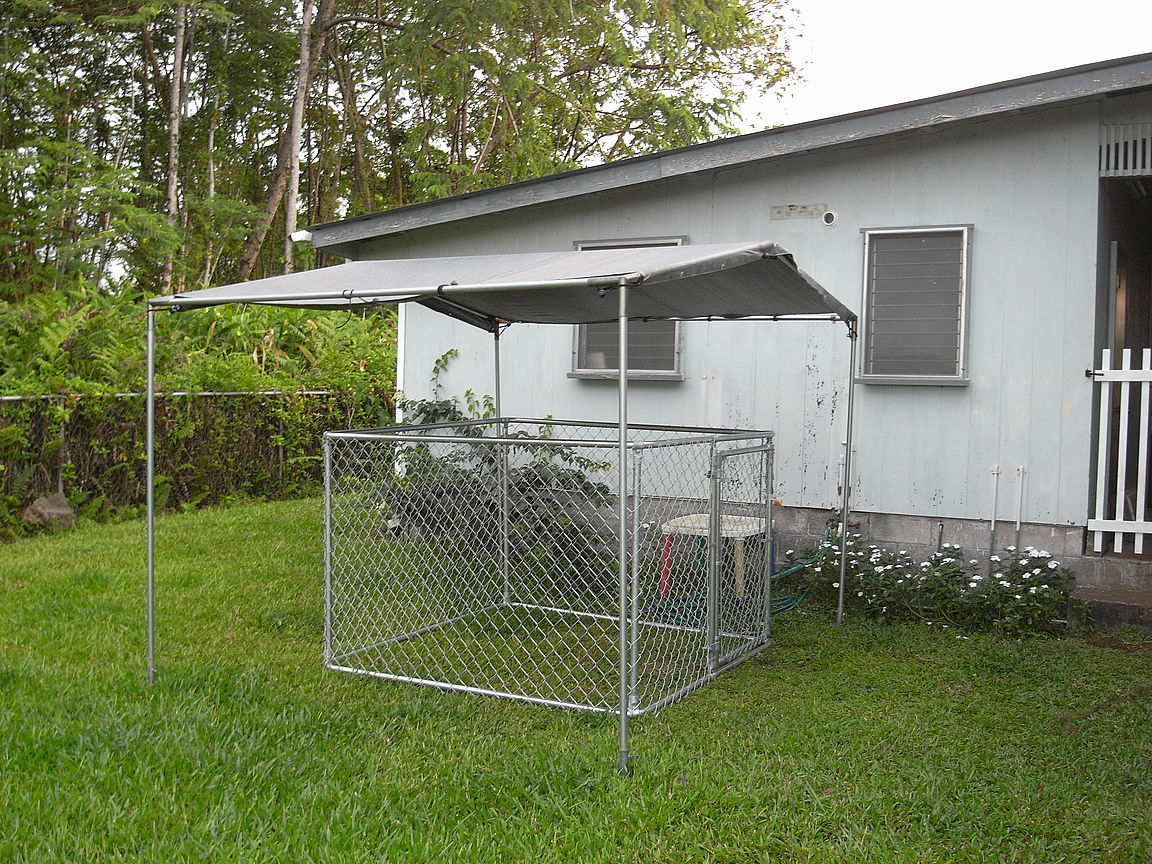
\includegraphics[width=8in]{R20090523-181340}

The 6x6x4 kennel seemed about the right size for 6 chickens, which is
what I was targeting.  My calculations were that six would yield us a
decent number of eggs per week.  After some reconsideration, we put the
coop up behind the annex.  I realized that I would probably rather keep
the chicks outdoors than in the annex, and this way they'd be closer to
the house to keep an eye on them while they were really small.  The nice
thing about using the kennel for a coop is that I could move it around
later, and thus get natural fertilizer all around the yard. 
\newpage

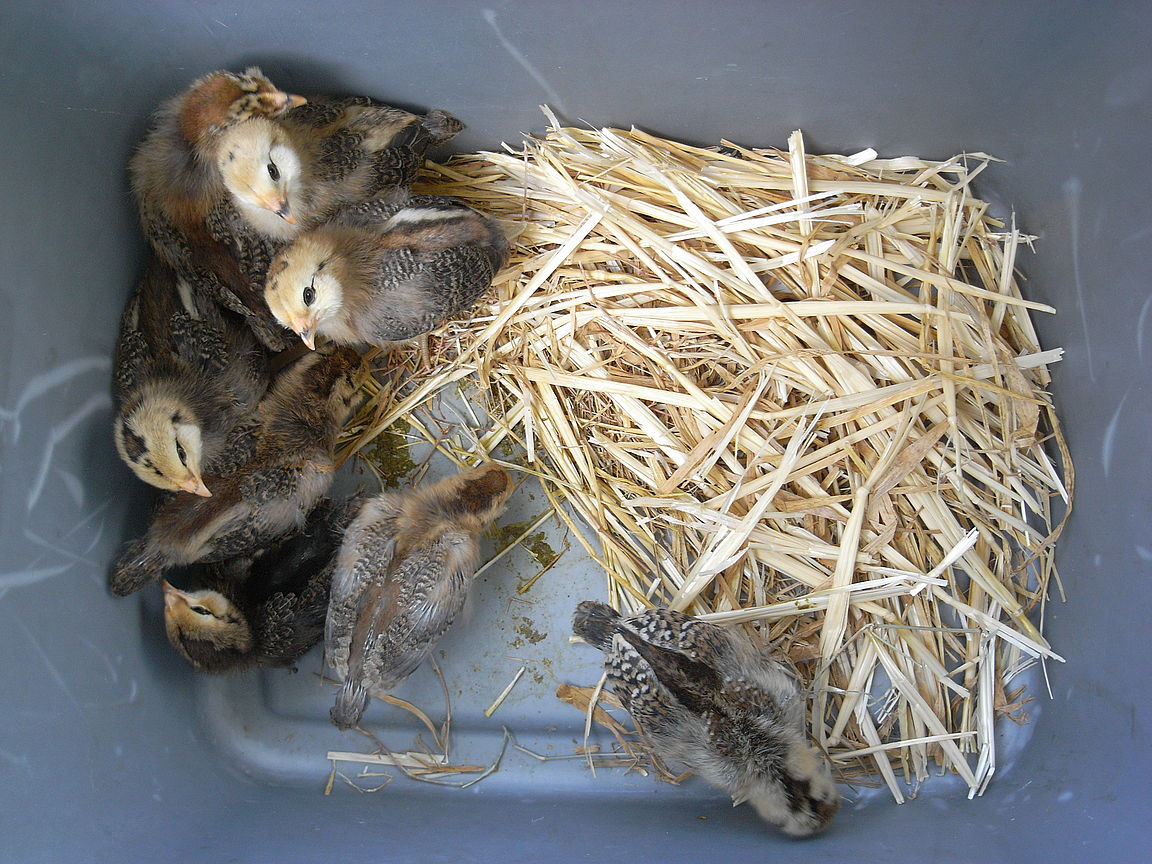
\includegraphics[width=8in]{R20090530-143901}

We went back to Del's a few days later, but the clerk informed me that
she'd sold the remainder of the chicks that morning to a single buyer,
and that they wouldn't be getting any more until next spring! Yikes! How
could we have let this happen?! After putting in a couple calls around,
I found out that the farm supply shop out in Pahoa still had a few
chicks on hand. I didn't recognize the type he mentioned when I asked,
but at this point, after buying all that stuff, I just wanted some
chicks. So I drove a half hour out and back to Pahoa Farm and Feed and
picked up 8 chicks, a bale of straw and a sack of feed. These chicks
looked more interesting than the Reds at Del's, and they were already
coming into feather. 
\newpage

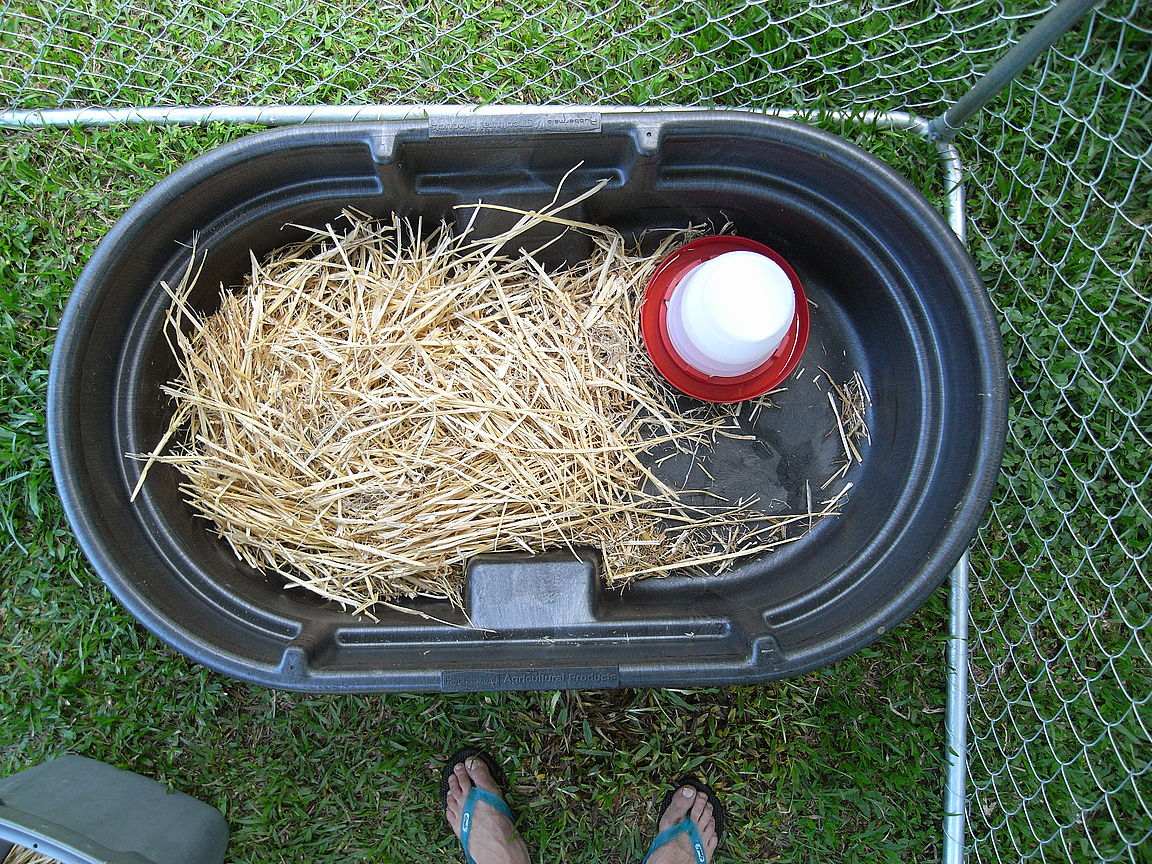
\includegraphics[width=8in]{R20090530-143924}

The chicks were going to need a cozy nest for the first few weeks, so I
took a tub that I had bought earlier from Del's for bathing our dog and
repurposed it as a nest.  That's the waterer on the right.  Chickens
need plenty of clean water. 
\newpage

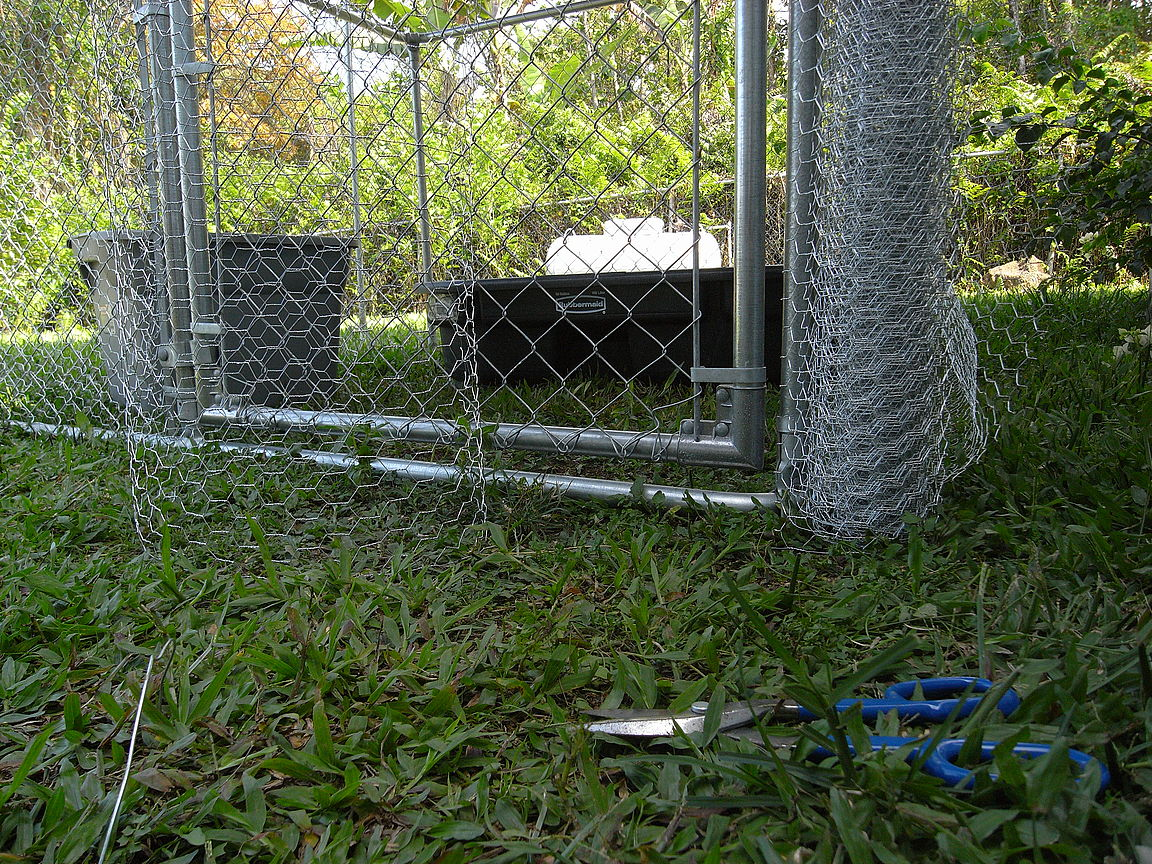
\includegraphics[width=8in]{R20090530-150204}

After taking a look at the size of the chain link fencing on the kennel,
I knew that it wasn't going to cut it as far as keeping the chicks in,
or predators out.  A cat maybe, but maybe not a mongoose or a rat.  So I
buzzed down to the old Home Despot and picked up a roll of 4x poultry
netting.  A quick wrap later, a few wire ties here and there and things
were looking more secure. 
\newpage

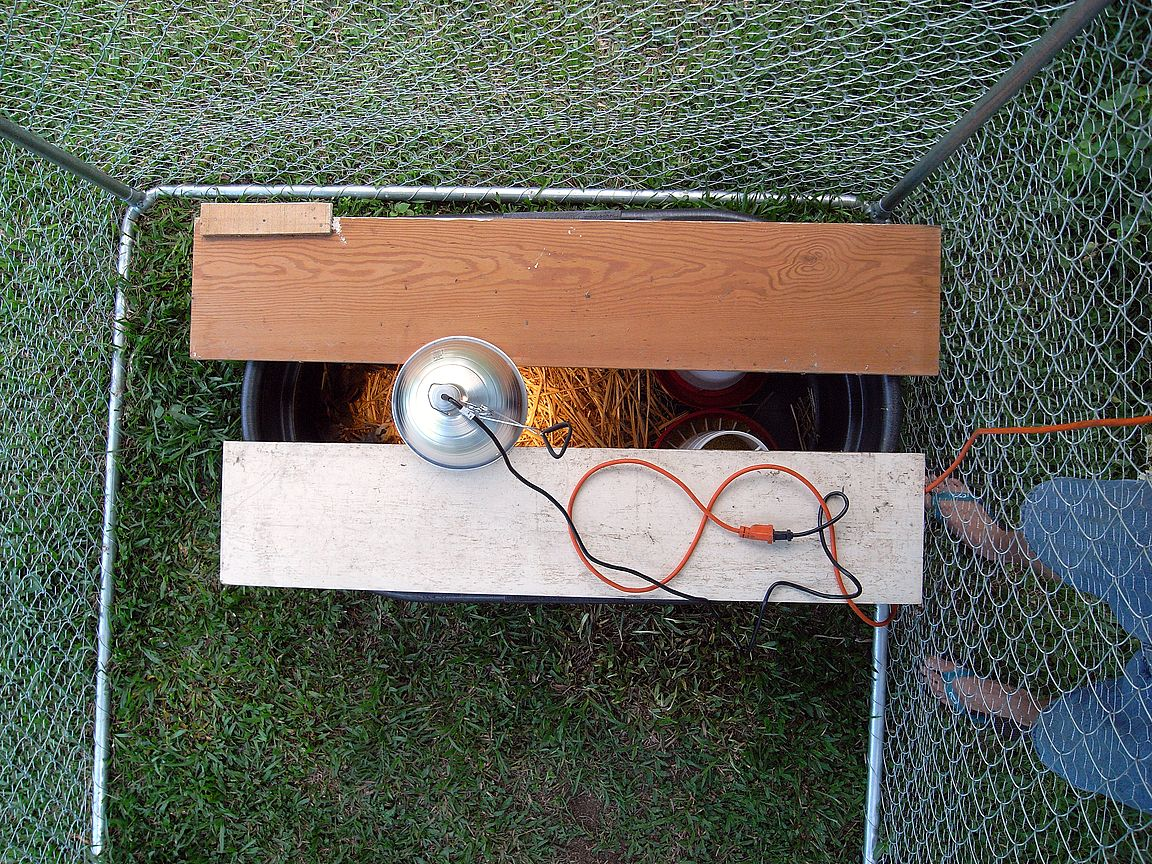
\includegraphics[width=8in]{R20090530-160556-levels}

I'd seen that the chicks had a light on at the farm supply, so I put out
an extension cord to the lamp that I'd bought.  Del's had said to use a
250W heat lamp, but out at Pahoa they were only using a 30W regular
incandescent.  Being summer in Hawaii and the chicks already in
feathers, I probably didn't need a light at all, but I screwed in a 60W
that I had around and figured they'd be OK.  Dropped the feeder inside,
laid two old boards across the top and everything was nice and cozy
inside for the little gals.  Later these boards would be completely
covered in manure.  In fact, everything would be! 
\newpage

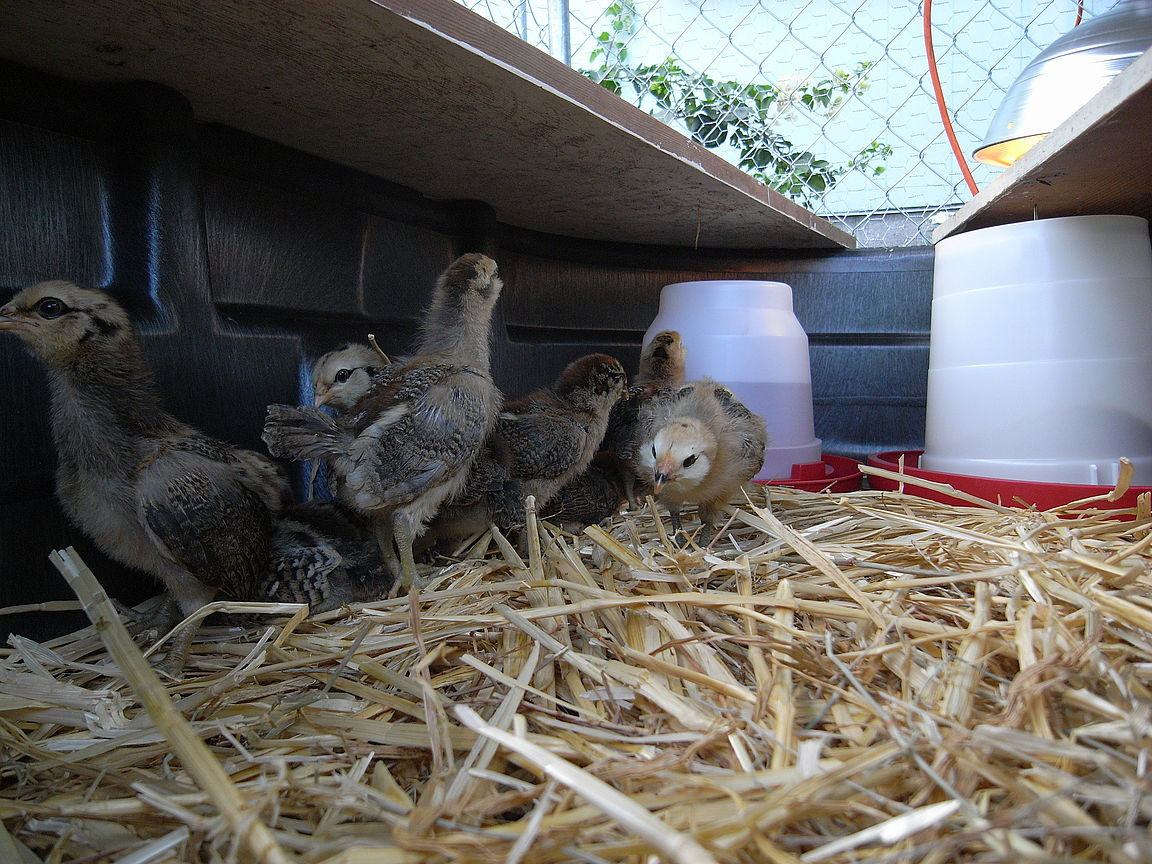
\includegraphics[width=8in]{R20090530-160824}

The chicks seemed right at home in the setup, and quickly found the
water and the feed. 
\newpage

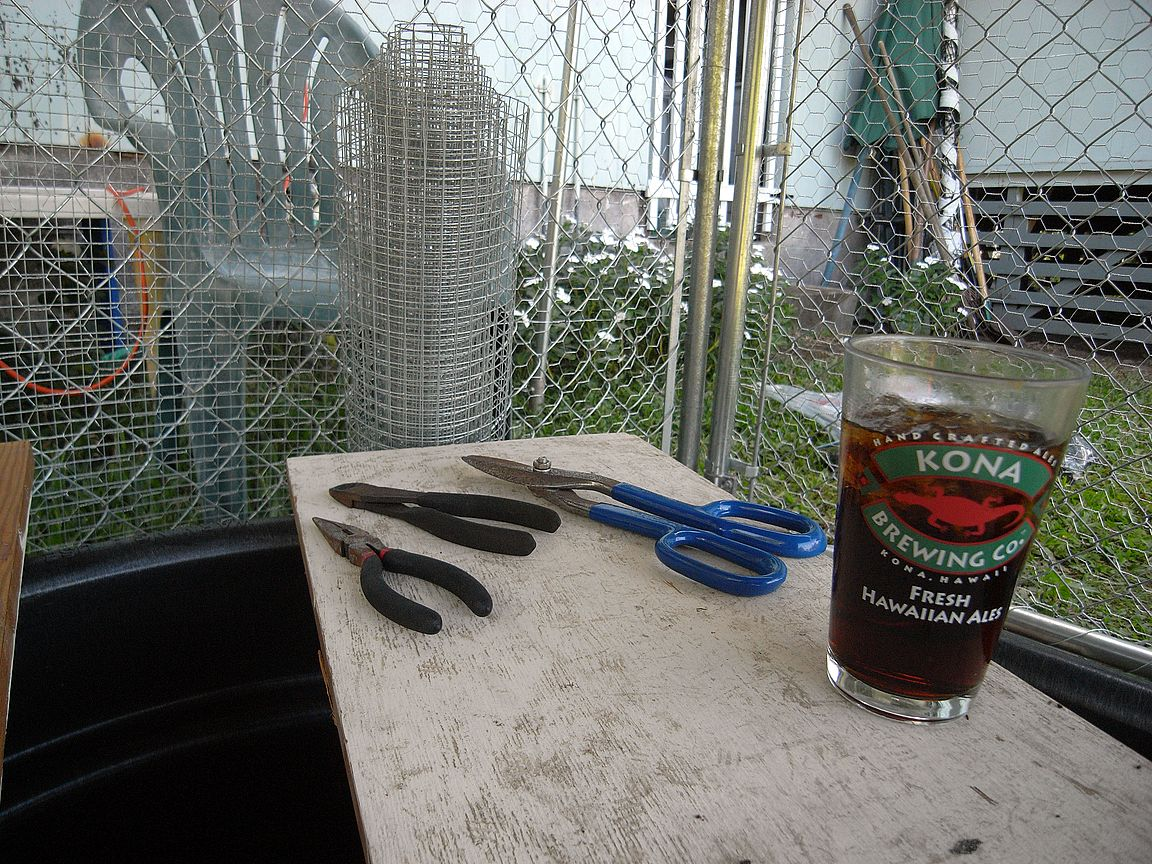
\includegraphics[width=8in]{R20090531-155246-levels}

After letting them run around the grassy part of the coop, I realized
that I might have to do even better than poultry netting when a couple
of them stuck their heads right through the holes.  I had visions of the
neighborhood cats pouncing, or our dog nipping, so back again I zipped
to the Despot, and grabbed a roll of 2x hardware cloth.  This I rolled
around the interior of the pen, and again wired it in with the kid's
help.  Now the chicks looked pretty darn secure, except for the top of
the kennel.  Tools (left ro right): needle-nose pliers, nips, tin snips,
rum and coke. 
\newpage

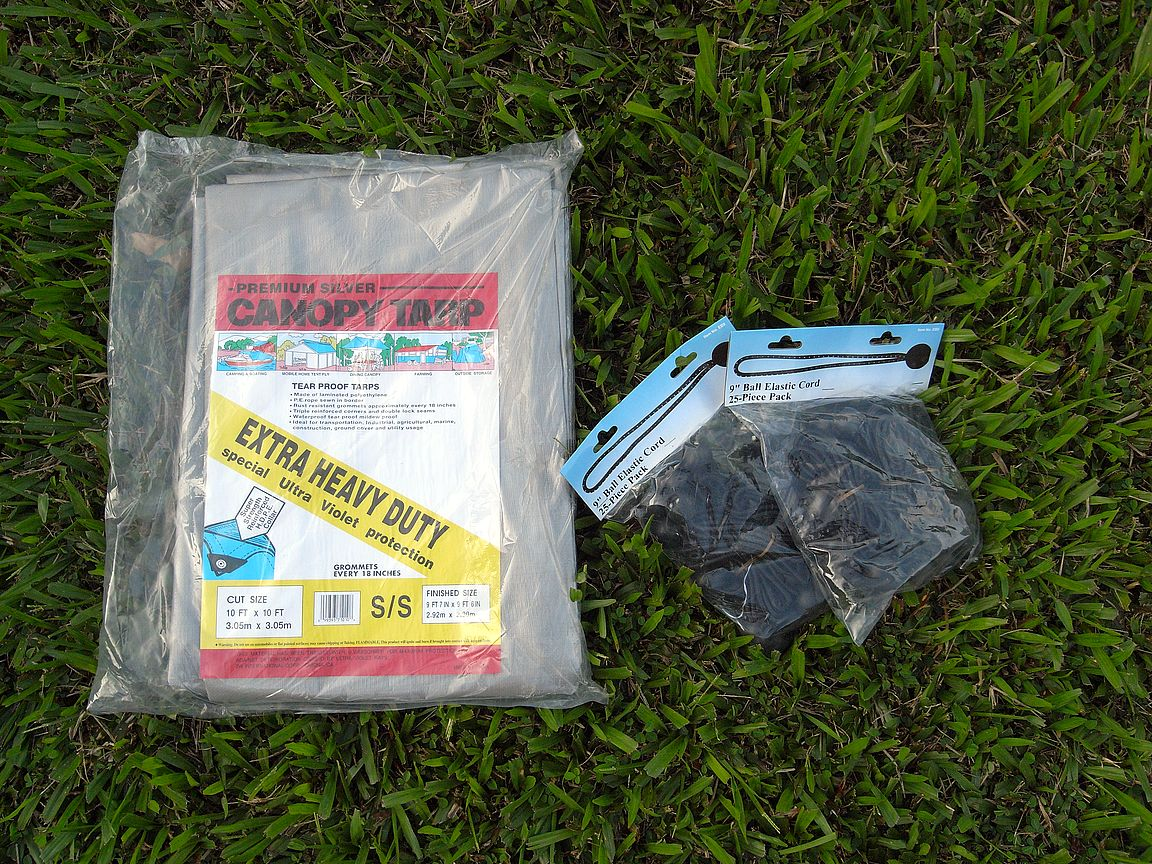
\includegraphics[width=8in]{R20090531-170420-levels}

The old tarp on the poles was ragged and had holes in it, so up went a
new 10x10 tarp. 
\newpage

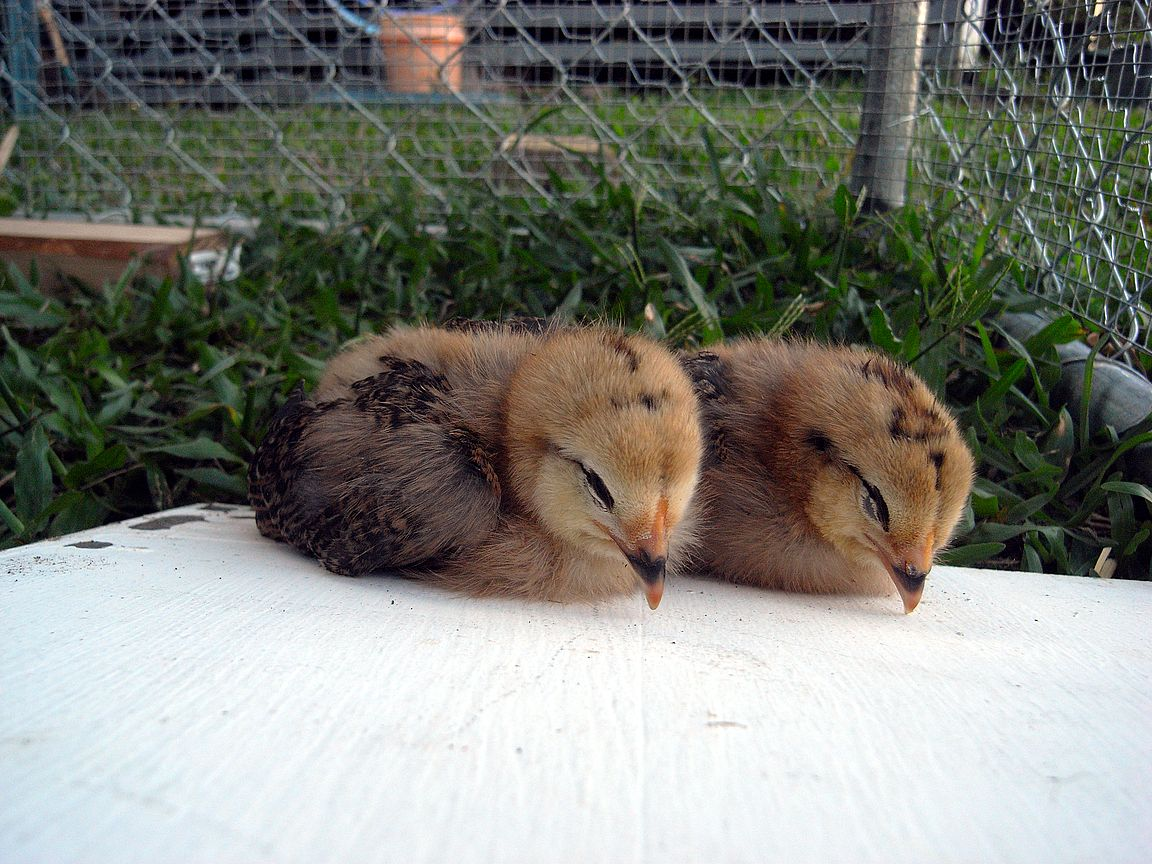
\includegraphics[width=8in]{R20090531-173219-master}

{\em Awwwww!}
\newpage

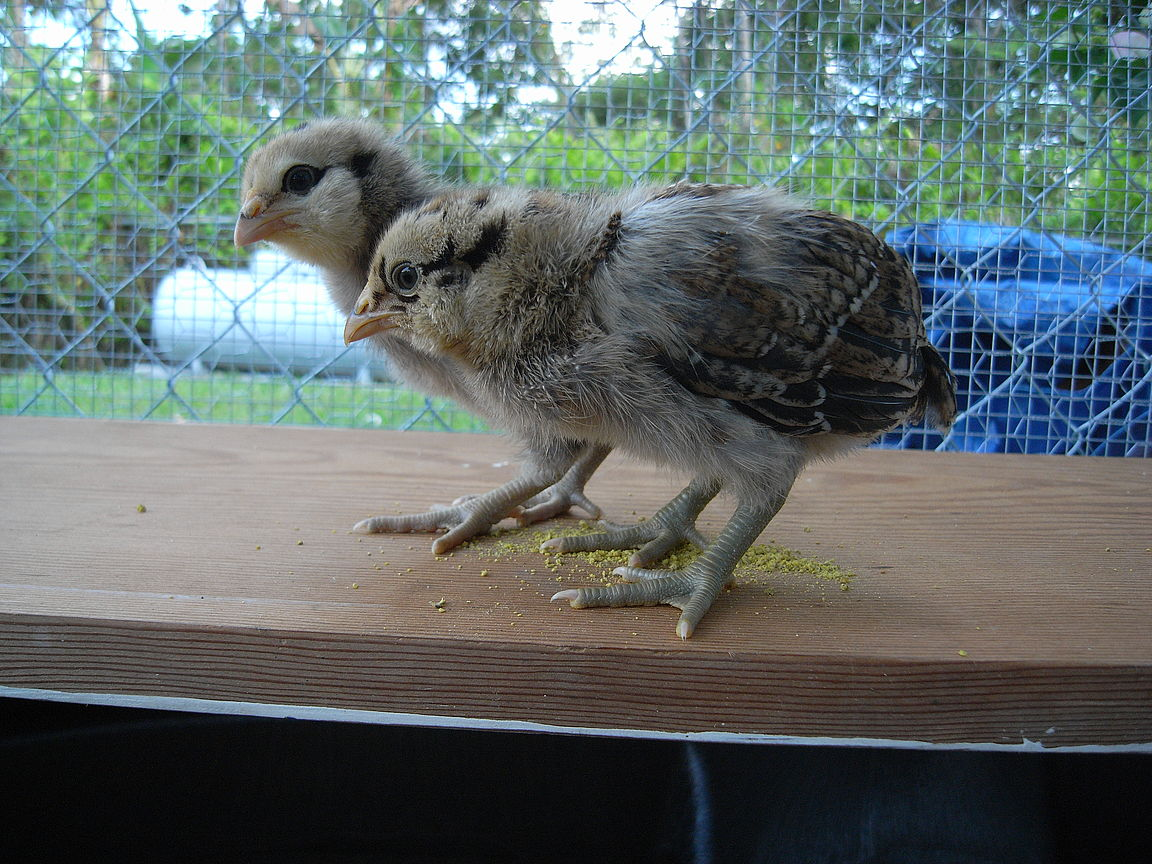
\includegraphics[width=8in]{R20090531-173505}

More {\em Awwwww!}
\newpage

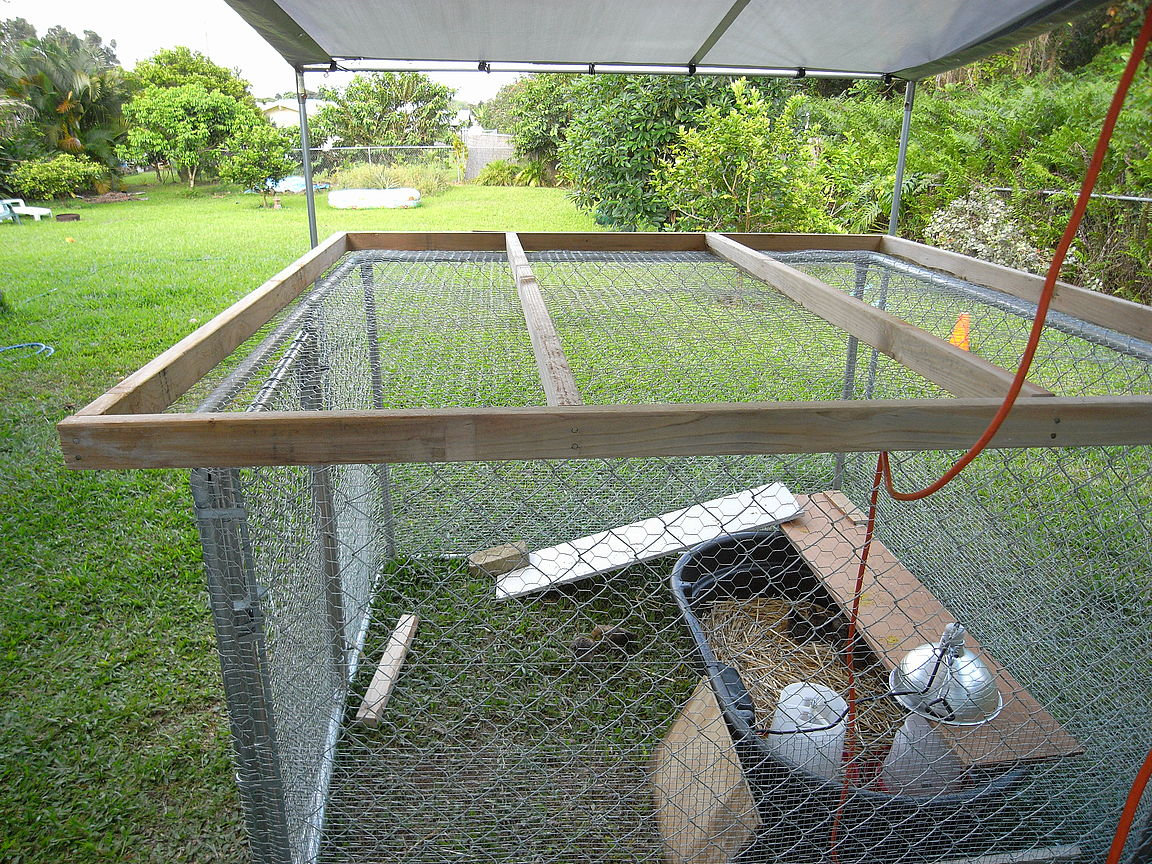
\includegraphics[width=8in]{R20090531-174207}

For the top, I fashioned a frame out of hibor 2x3's and using a staple
gun, tacked some poultry netting to the frame.  This then rested on the
top of the kennel.  Home Depot was really making a dent in my wallet!
At least I was confident that the chicks would be safe while they were
inside. 
\newpage

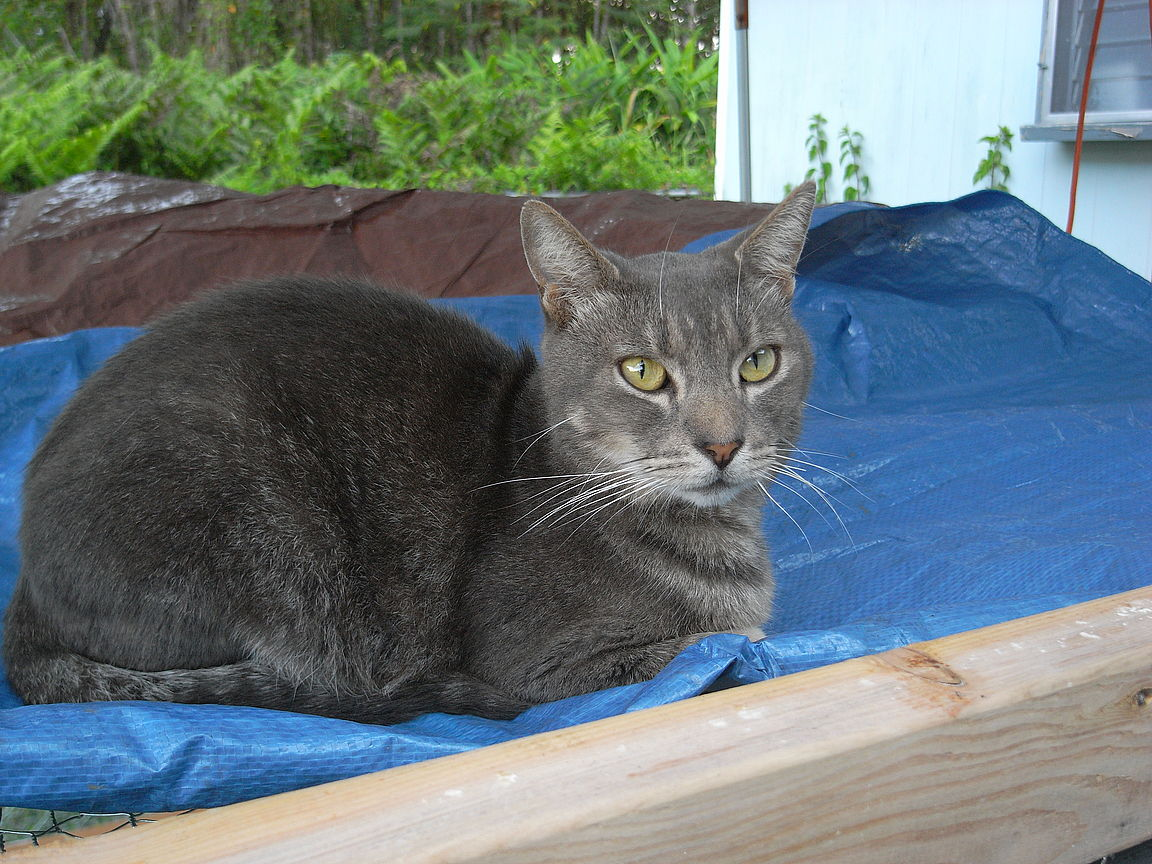
\includegraphics[width=8in]{R20090531-175613}

Just in time!  Our cat Jasper made an appearance and made himself
comfortable on top of the coop.  He didn't seem all that interested in
the chickens.  Little did we know, that he would die only a week later
of some sort of poisoning, possibly the neighbor's extensive Roundup
treatment. 
\newpage

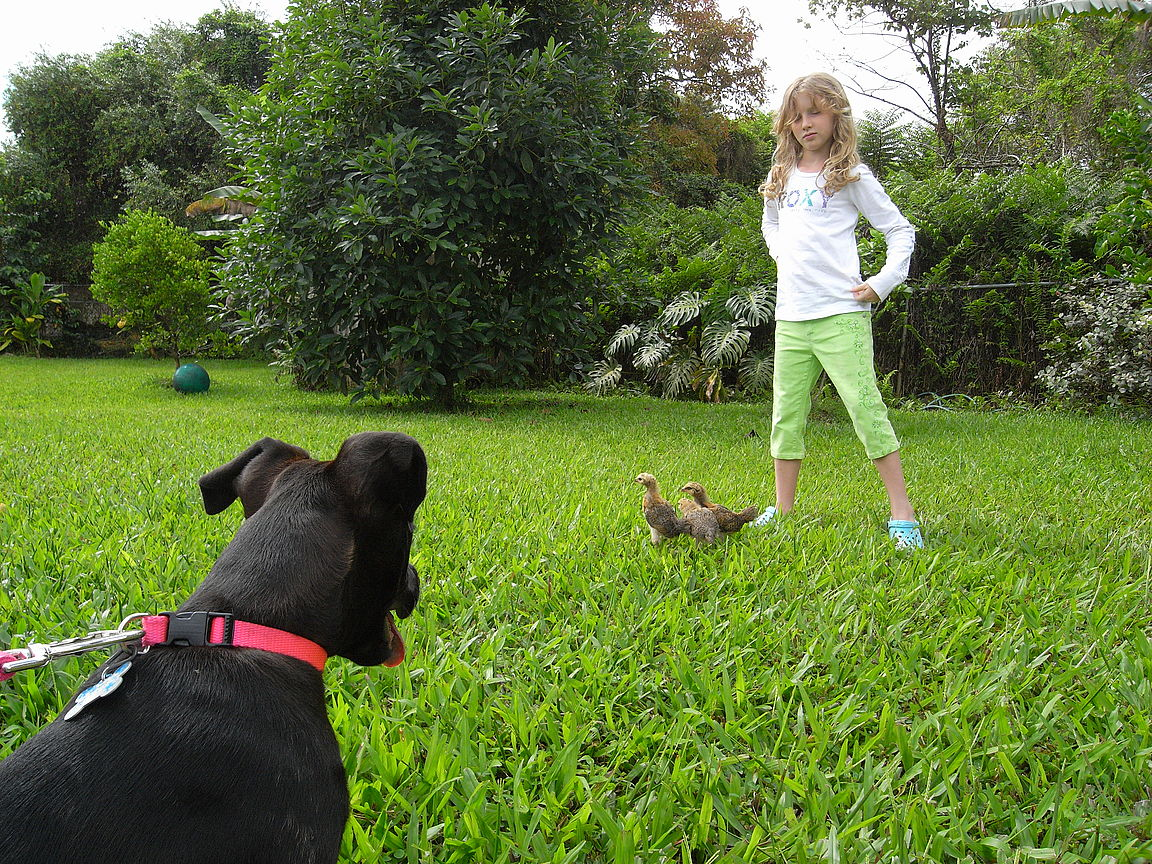
\includegraphics[width=8in]{R20090606-093158}

The real question was how our dog Lily would react to the chickens.  We
really need her to be at ease with them, because the plan is to
eventually let the chickens out in the backyard to forage during the
day, and come back to the coop at night.  She was facinated by the
chicks and would chase them around the outside of the coop.  Not good.
A week or so went by and we decided to give her some supervised visits
with them in the yard. 
\newpage

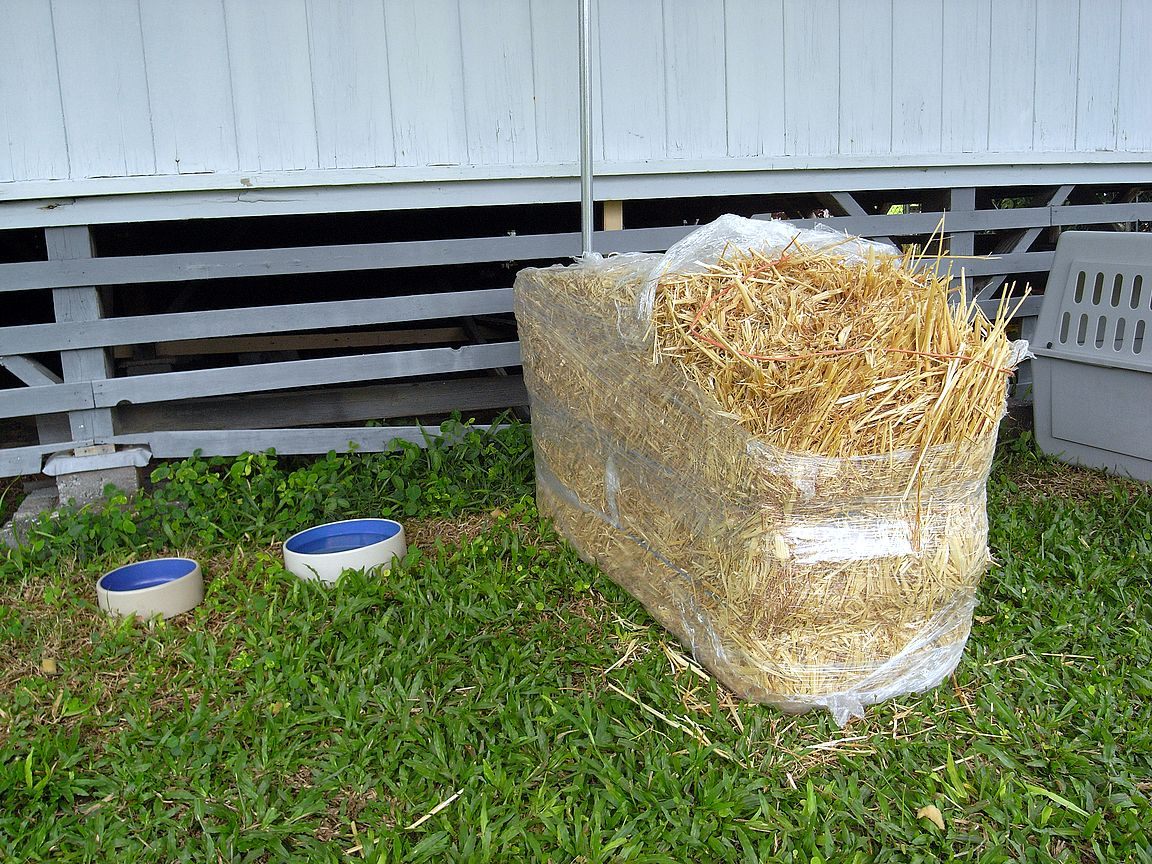
\includegraphics[width=8in]{R20090606-145351-levels}

The chickens get fresh water every day, more feed every couple of days,
and new straw every few days.  This straw bale should last for a
while... 
\newpage

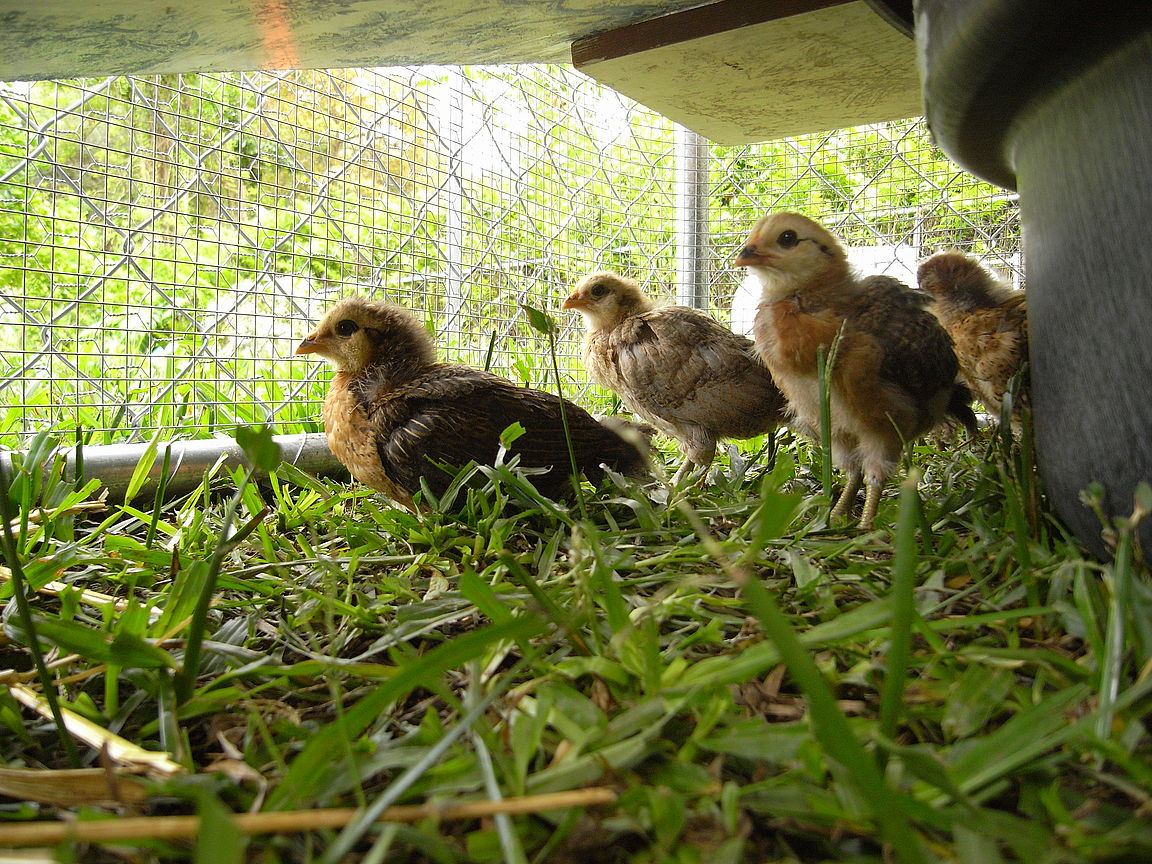
\includegraphics[width=8in]{R20090606-150039}

A few days after moving in the chicks seem happy and healthy.  They are
eating well and have taken to hopping in and out of the nest as they
like and running around the coop, pecking at everything.  Feathers are
coming in fast. 
\newpage

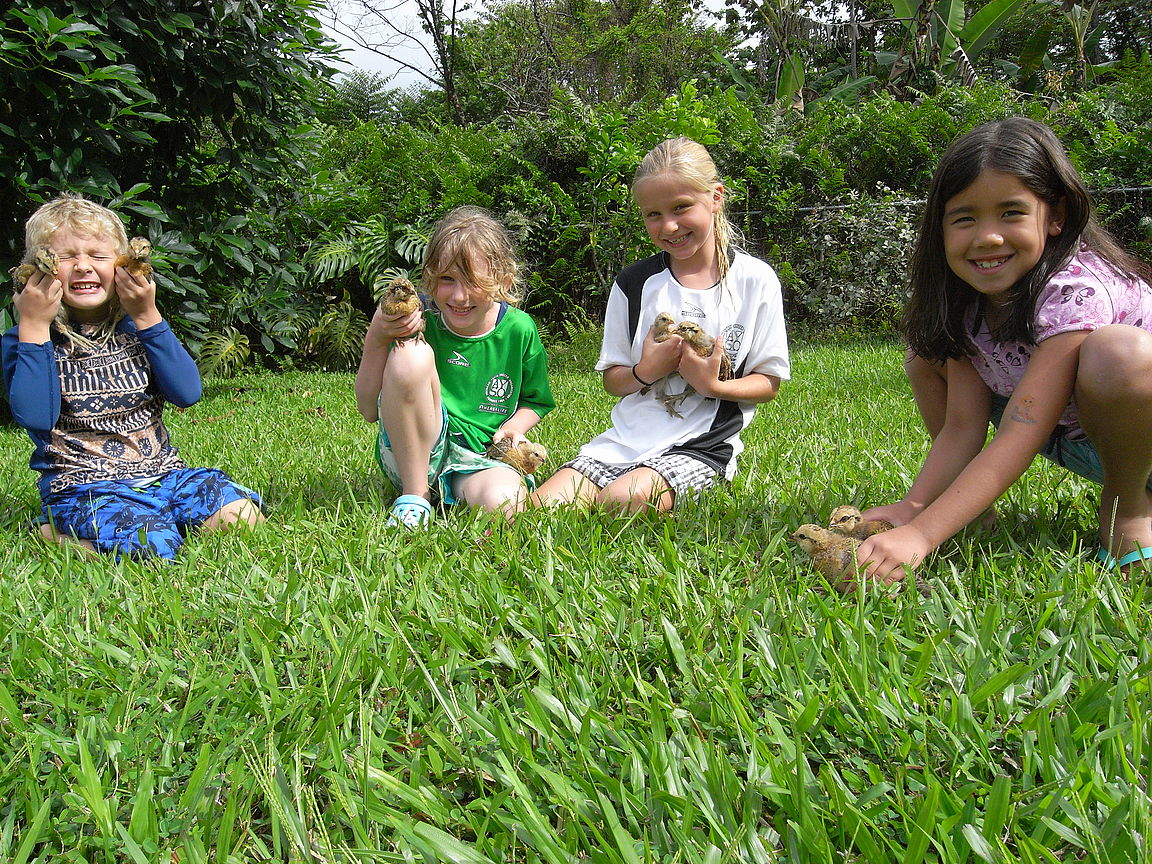
\includegraphics[width=8in]{R20090606-151823}

Left to right: Tyler with Snape and Voldemort, Momi with Furrow and
Harry Potter, Lori with Junior Junior and Hermione and Siena with Junior
and Ron Weasley.  Yes, they are named after Harry Potter characters,
with a few exceptions. 
\newpage

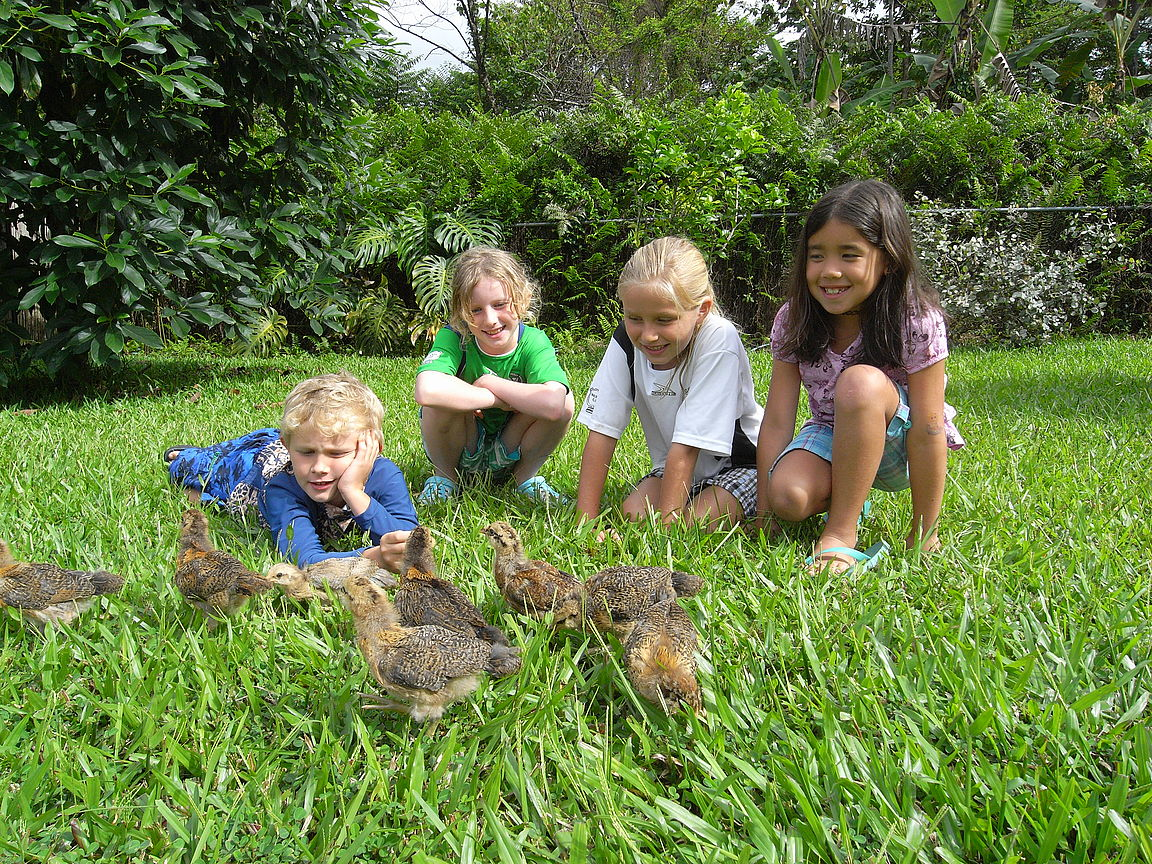
\includegraphics[width=8in]{R20090606-151907}

We are now regularly letting them come out of the coop to get used to
the idea of foraging and then returning home.  Already they have a
strong attachment to the coop. 
\newpage

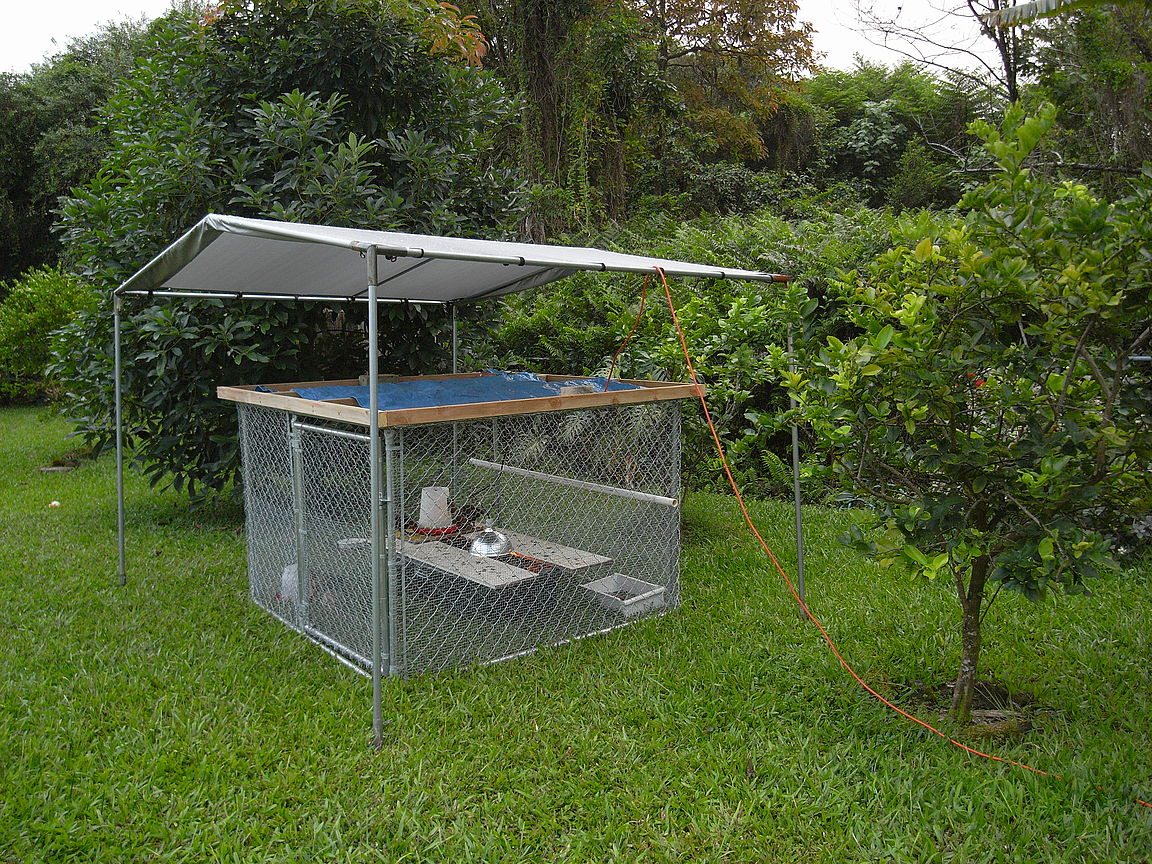
\includegraphics[width=8in]{R20090611-181412}

After another week, it was beginning to get a bit fragrant at times near
the house, if the breeze happened to blow the right way.  We decided to
move them out a little farther into the yard, to a fresh patch of grass.
Sandwiched between the lime, lemon and advocado trees seemed like a good
spot.  Here the coop design proved it's worth, as we could move the
whole thing in a matter of minutes.  I began to see the attraction of
the ``chicken tractor'', or coop built on wheels... 
\newpage

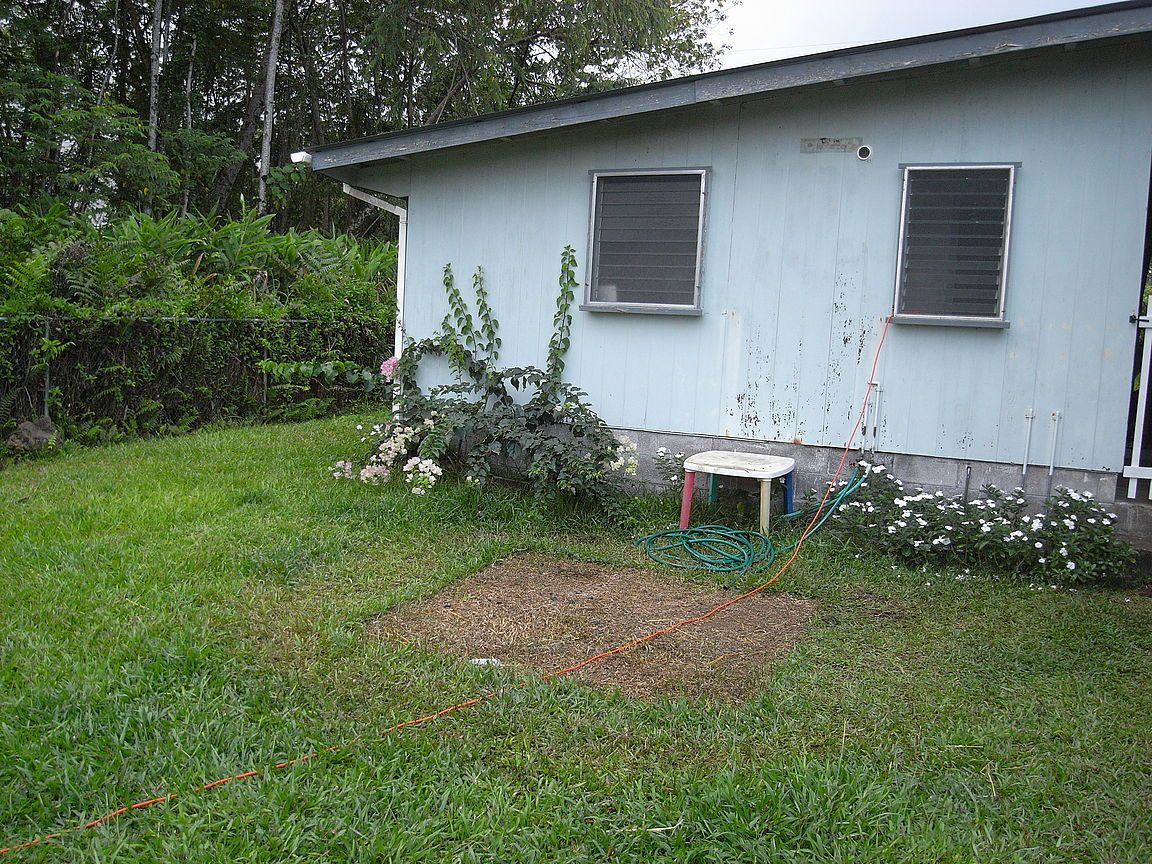
\includegraphics[width=8in]{R20090611-181347}

Another reason for the move was that they basically had denuded the spot
they were in.  But with a potent mix of Hawaii sunshine, Hilo rain and
plenty of chicken crap in the grass, it will come back in no time. 
\newpage

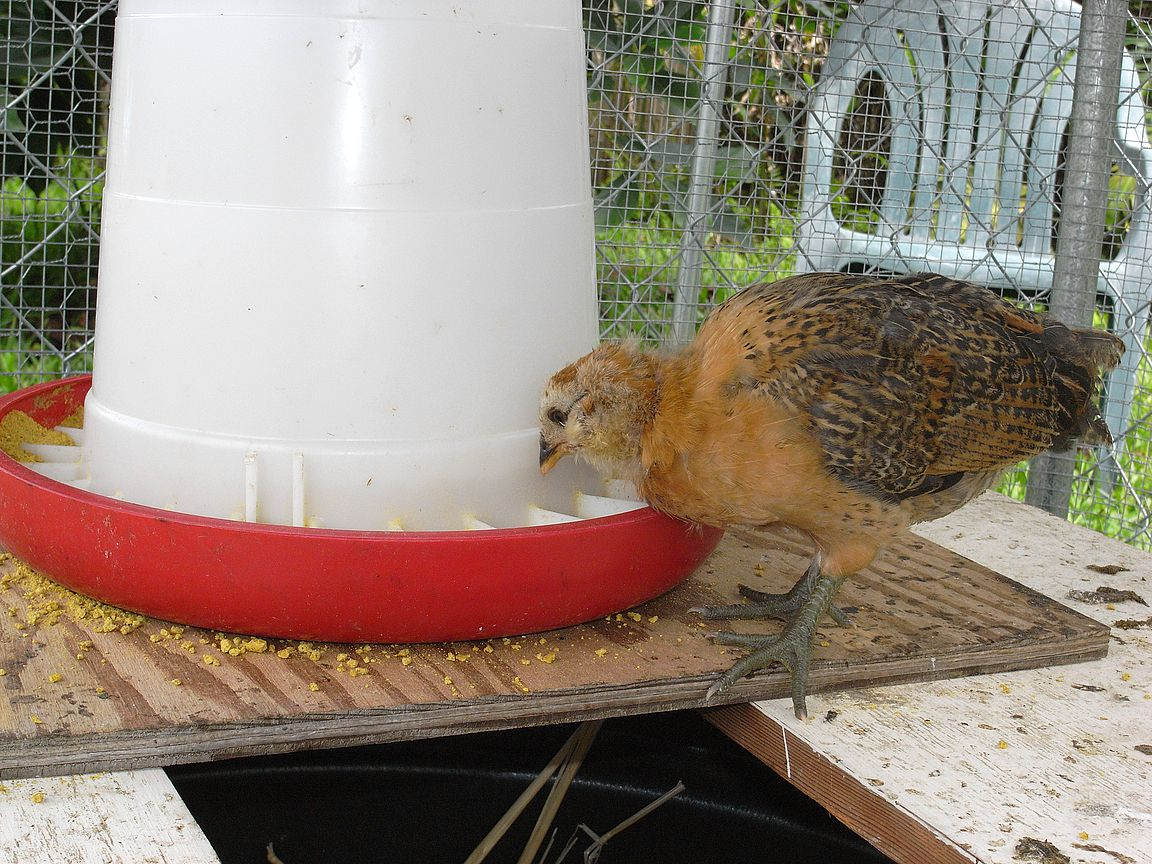
\includegraphics[width=8in]{R20090612-133412-levels}

By now the chicks are growing at an unbelievable rate.  Their plumage
and markings begin to take on the appearance of how they will look as
adults.  These were sold as ``Araucanas'', a kind of chicken originally
from Chile, however a little research on the net revealed that ours are
probably ``Ameraucanas'' or maybe even regular ``Easter Eggers''.  
\newpage

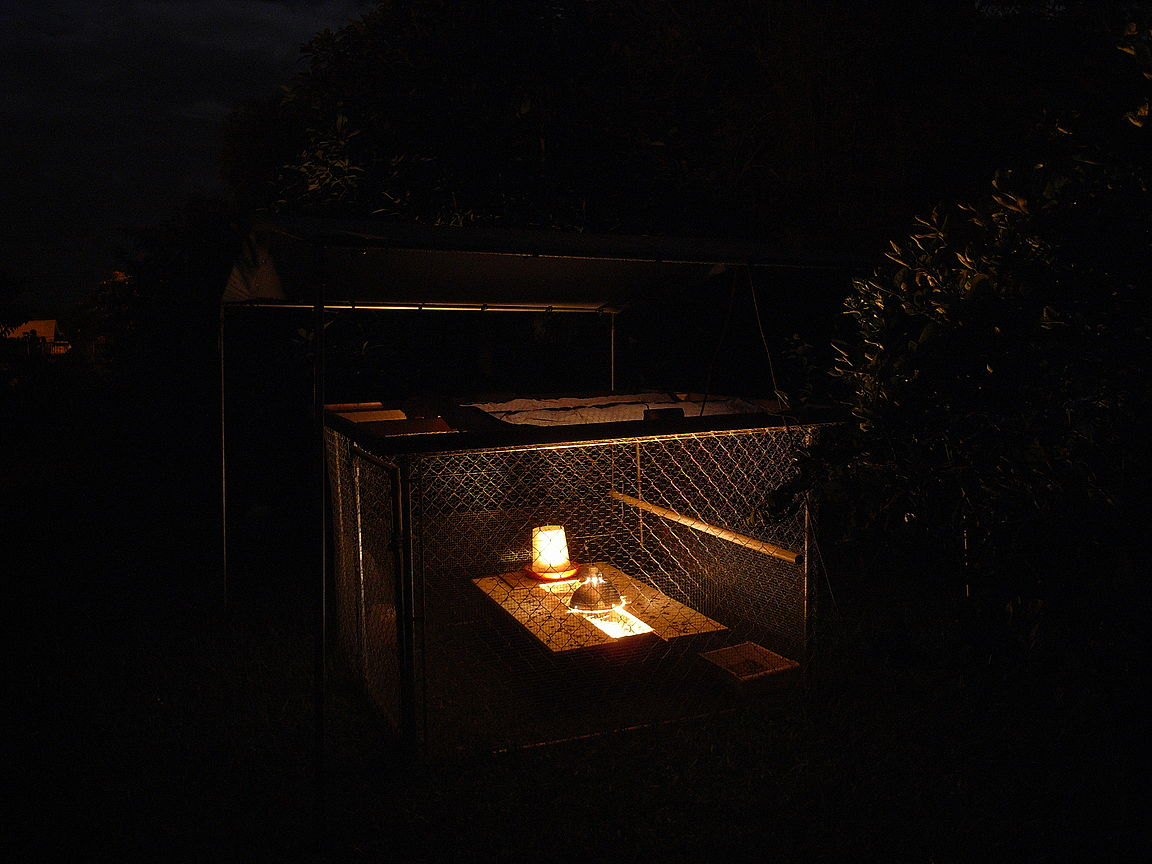
\includegraphics[width=8in]{R20090613-013821}

The coop at night.  You can see the roosting bar I put in for them on
the right side.  Apparently chickens like to roost.  Who'd have thunk
it?  At this point I also pulled the waterer and feeder out of the
nesting area, since they seem to have no trouble finding it outside the
nest, and it gives them a little extra room inside.  I'll probably start
leaving the light off at night now, since they seem to be filling in
feathers nicely. 
\newpage

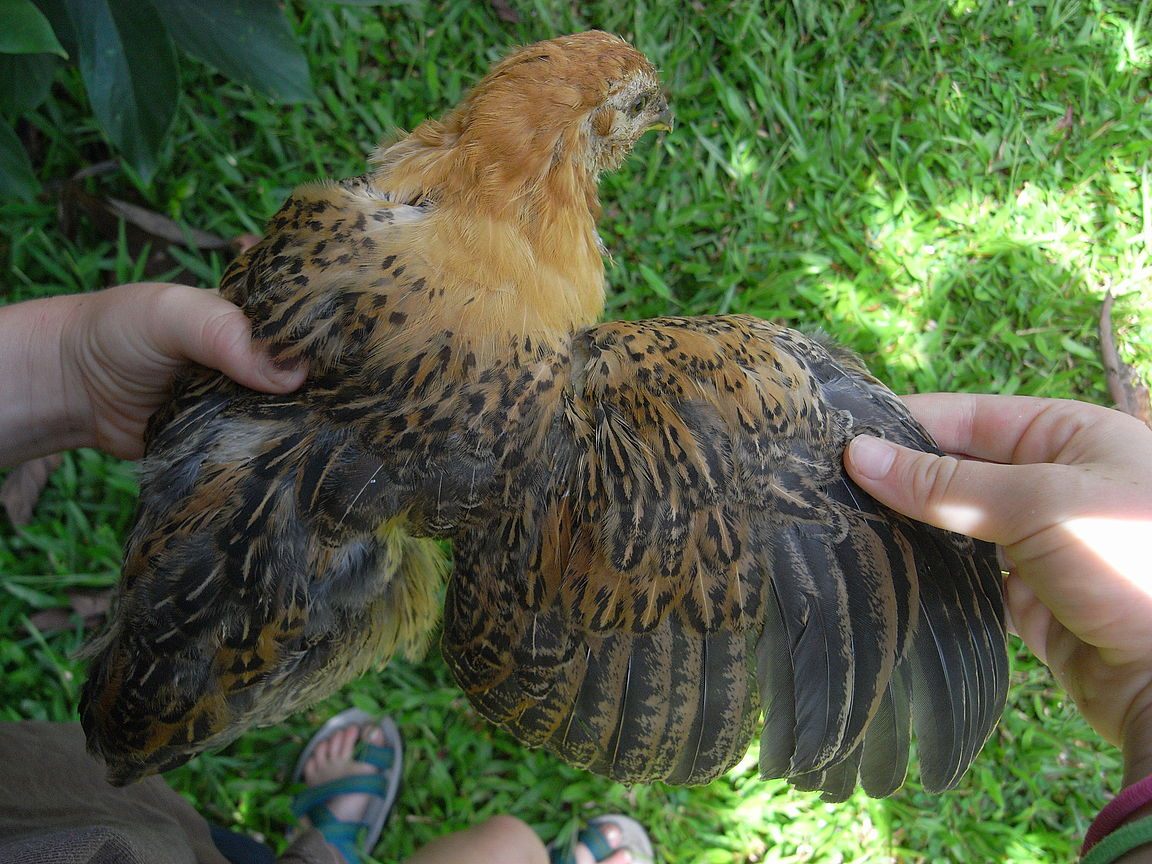
\includegraphics[width=8in]{R20090619-102140}

I've been thinking about clipping wings.  They are getting pretty good
at flapping and doing short little hop flights here and there.
Supposedly I can just clip the outer 10 ``flight feathers'' on one side,
which makes them unbalanced in flight.  I think they may need to be a
little older first. 
\newpage

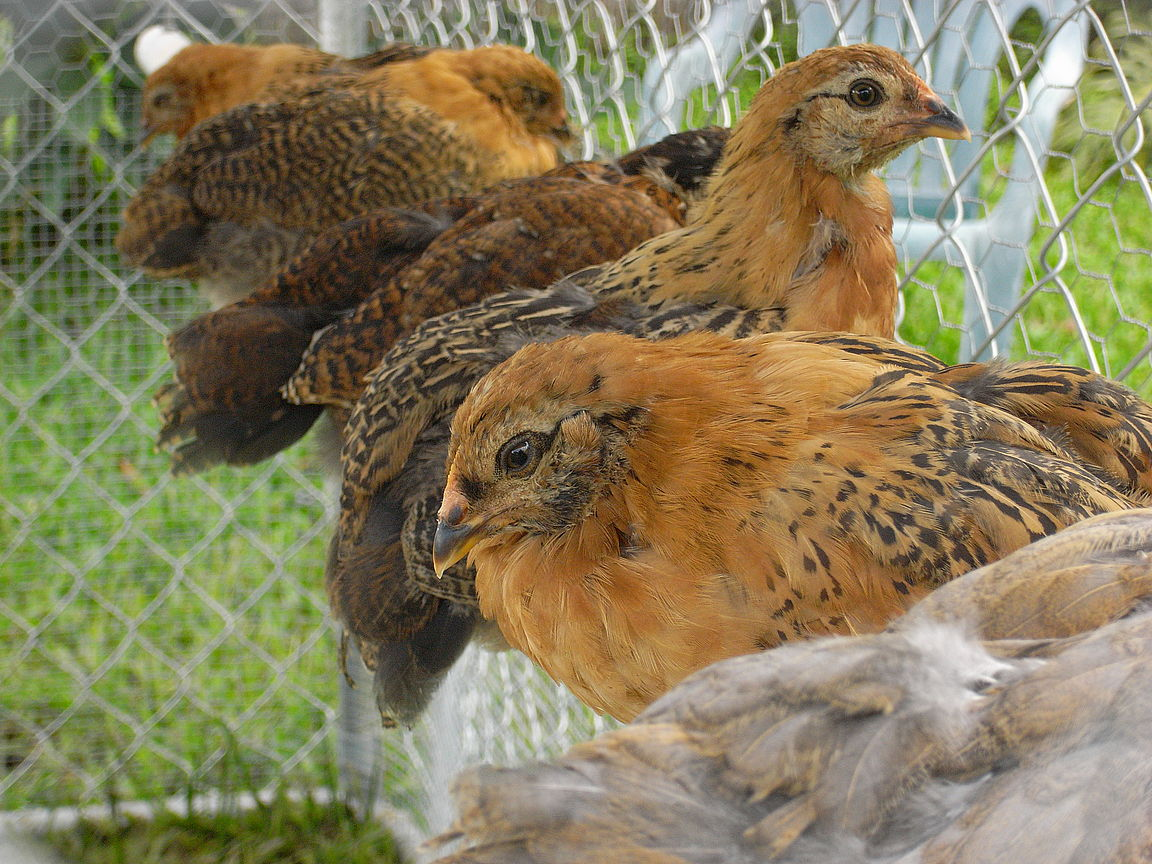
\includegraphics[width=8in]{R20090619-103748}

The chickens (it seems strange to call them chicks now, they are so big)
are really getting fond of foraging now.  We still can't let them out of
the pen unsupervised though; they're not quite big or bold enough yet.
One morning when I went out to feed and water them a cat was sitting
there with his face right up to the cage, watching. 
\newpage

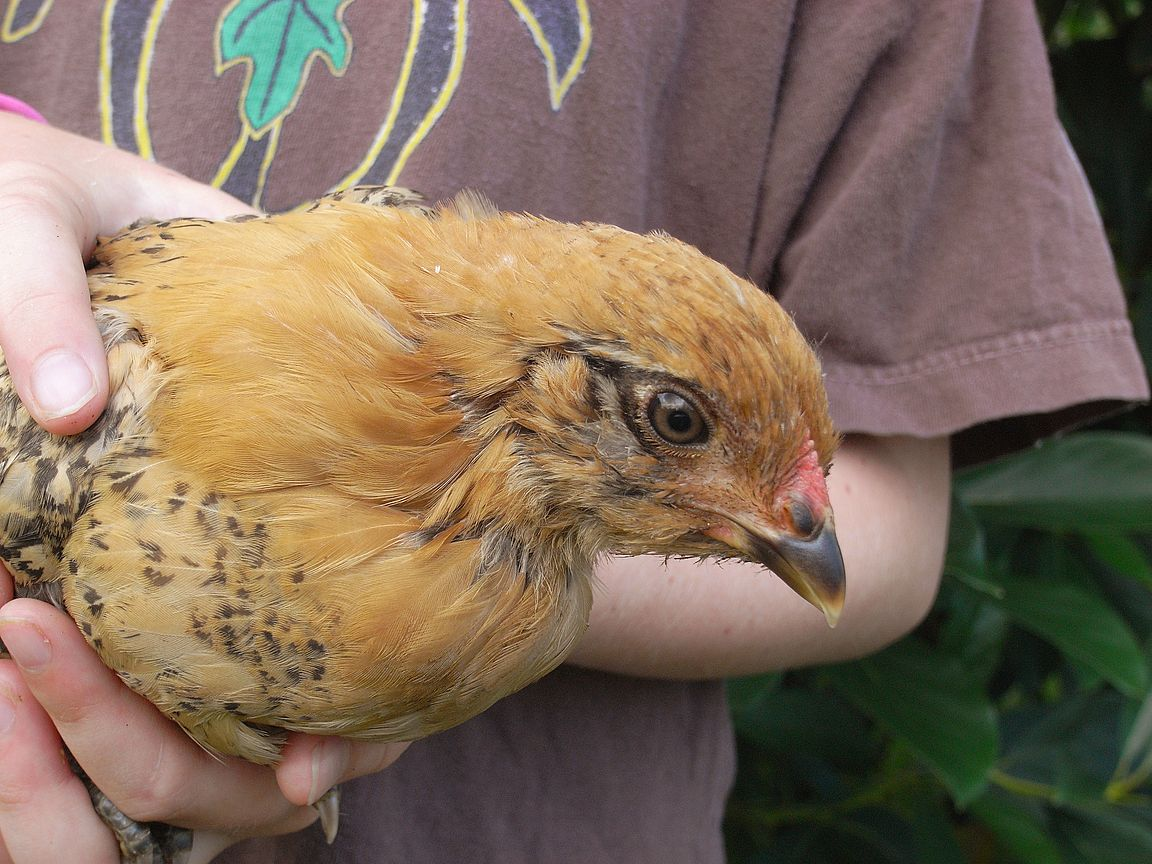
\includegraphics[width=8in]{R20090619-101312-curves}

\begin{center}{\Large ``Furrow'' }\end{center}
\newpage

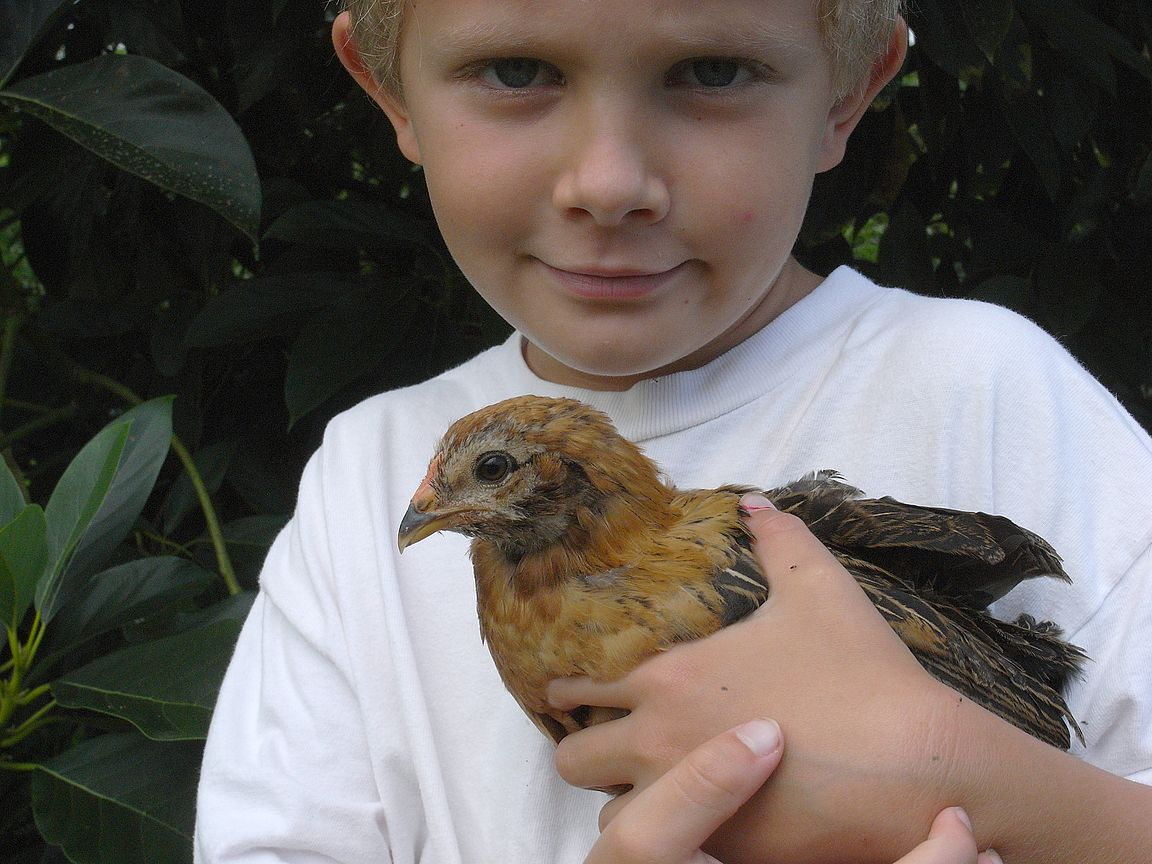
\includegraphics[width=8in]{R20090619-101502-levels}

\begin{center}{\Large ``Voldemort'' }\end{center}
\newpage

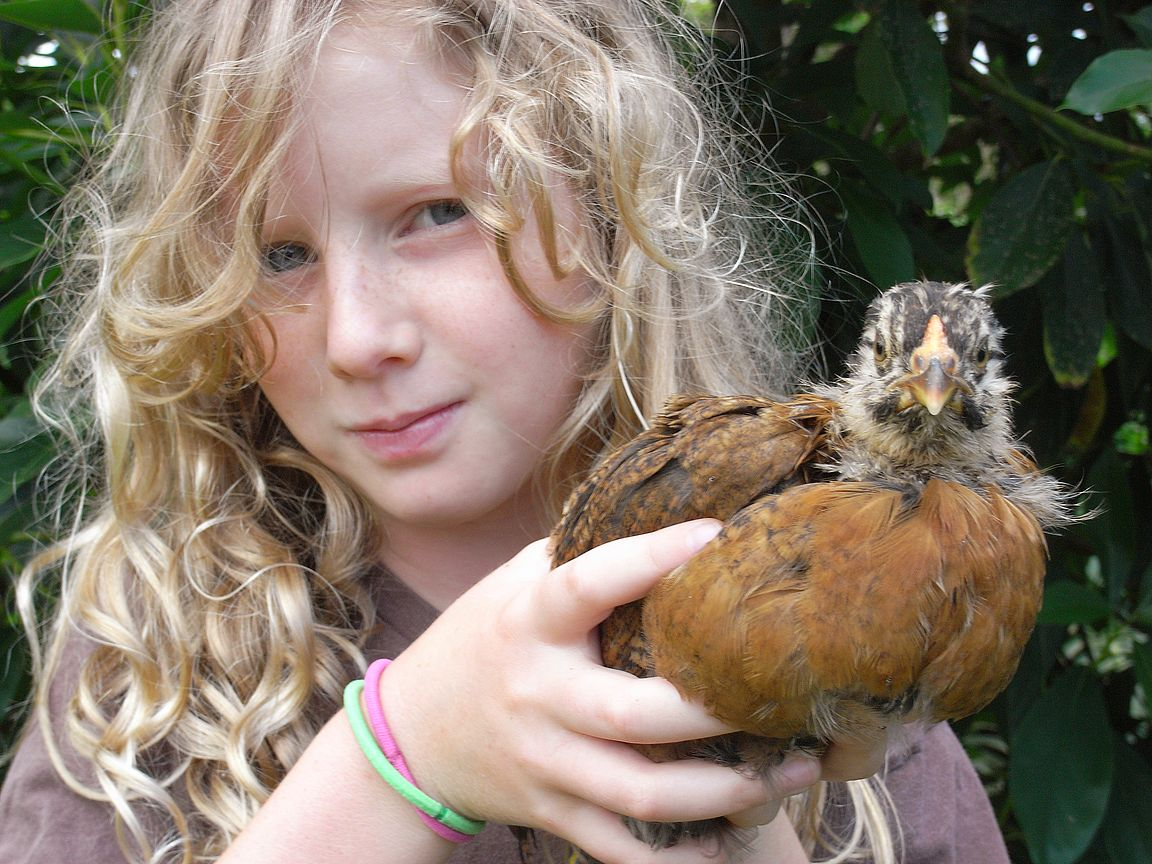
\includegraphics[width=8in]{R20090619-101707-curves}

\begin{center}{\Large ``Hermione'' }\end{center}
\newpage

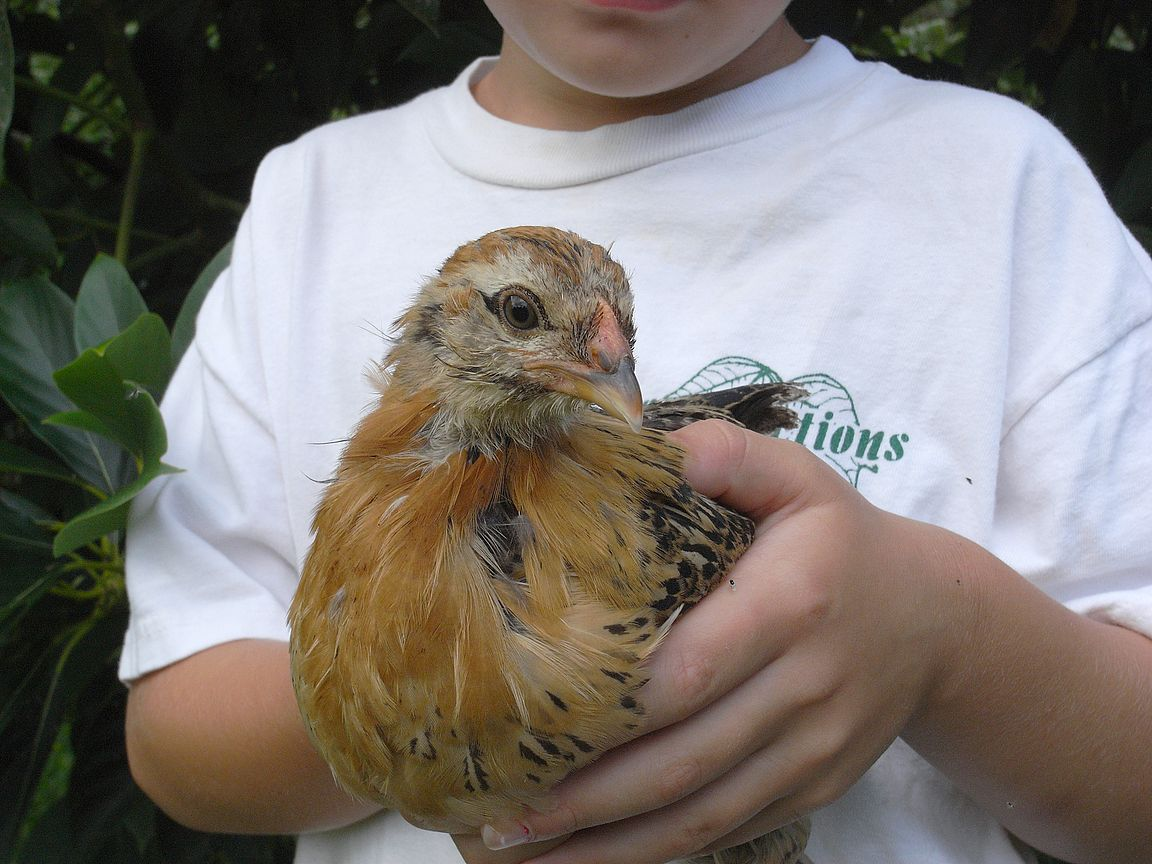
\includegraphics[width=8in]{R20090619-101832-levels}

\begin{center}{\Large ``Severus Snape'' }\end{center}
\newpage

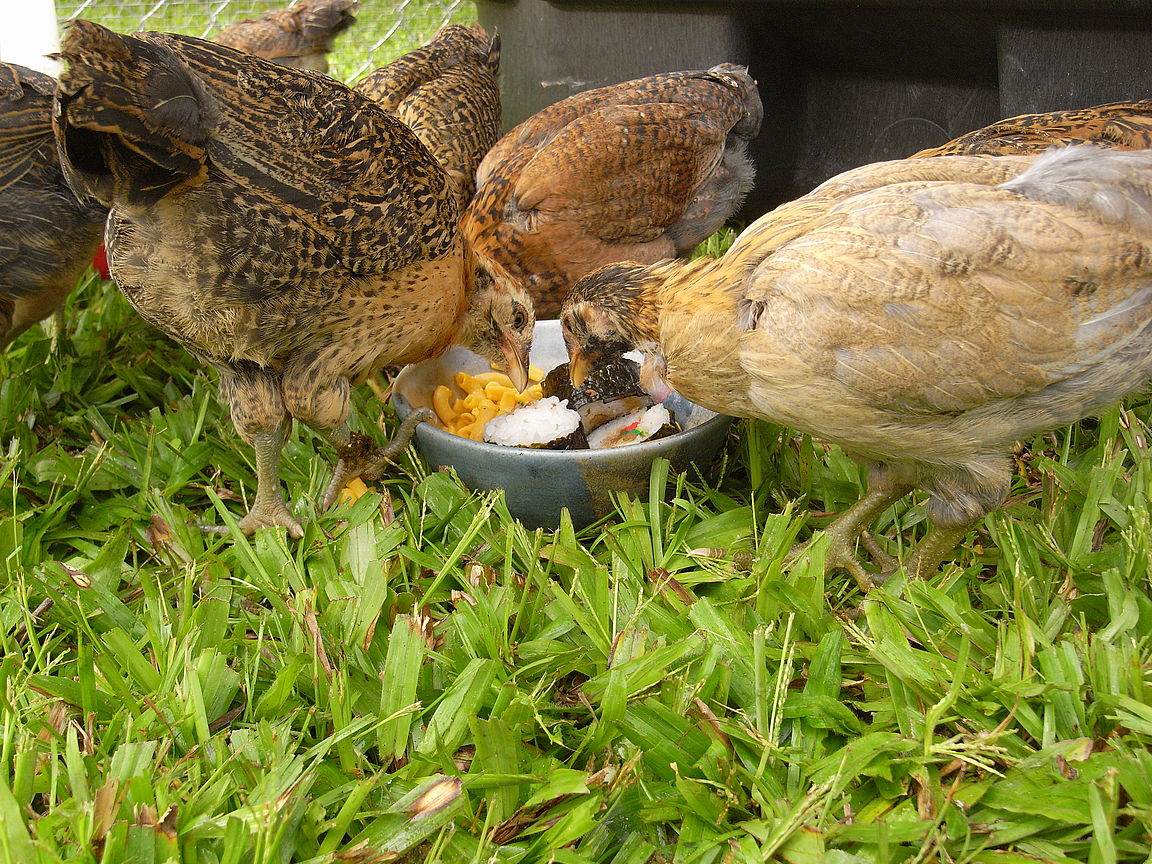
\includegraphics[width=8in]{R20090620-094747}

My coworker Alan says that chickens like compost.  So I started giving
them some table scraps.  They really seem to like tortillas.  Which is
good, because we make a lot of quesadillas.  They go berserk when I open
the door and toss in the bits.  They also, strangely, love bananas.
\newpage

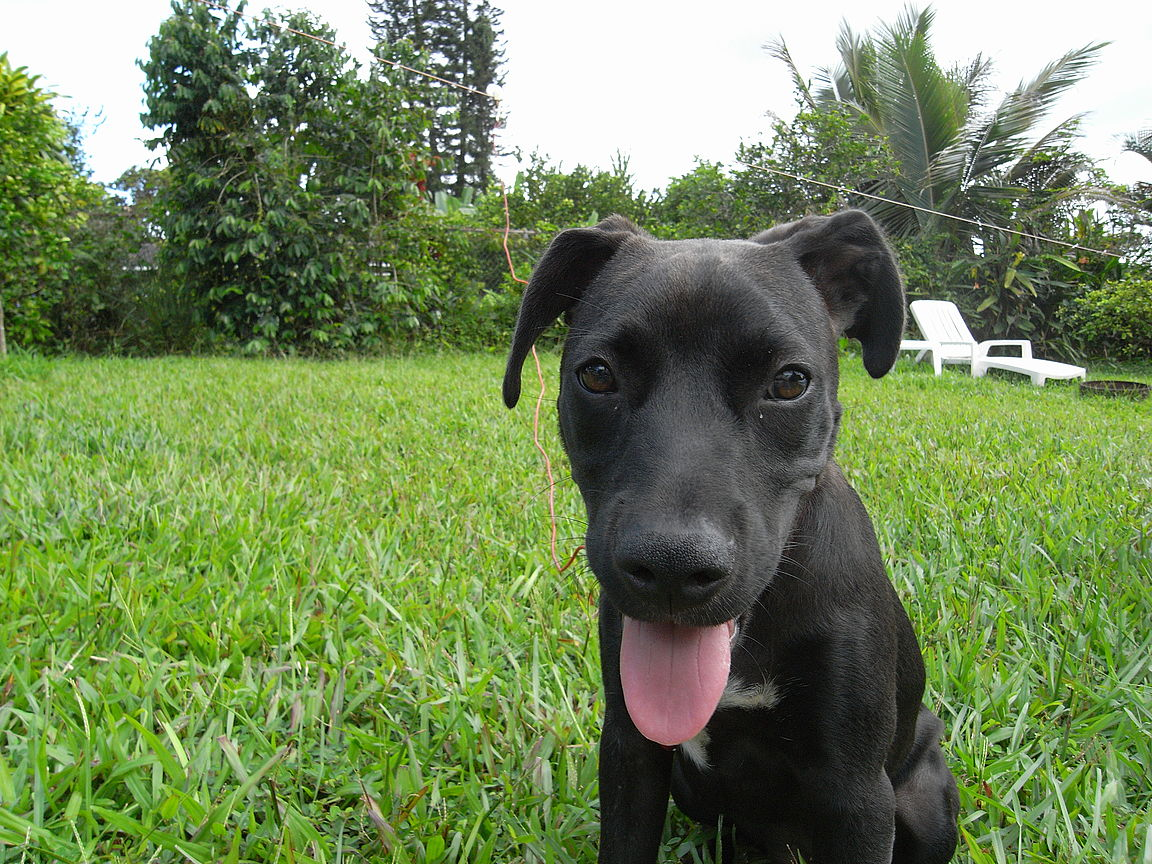
\includegraphics[width=8in]{R20090619-103104}

``Do I look like I'd harm a feather on their soft little heads?''  Well,
yes, actually. 
\newpage

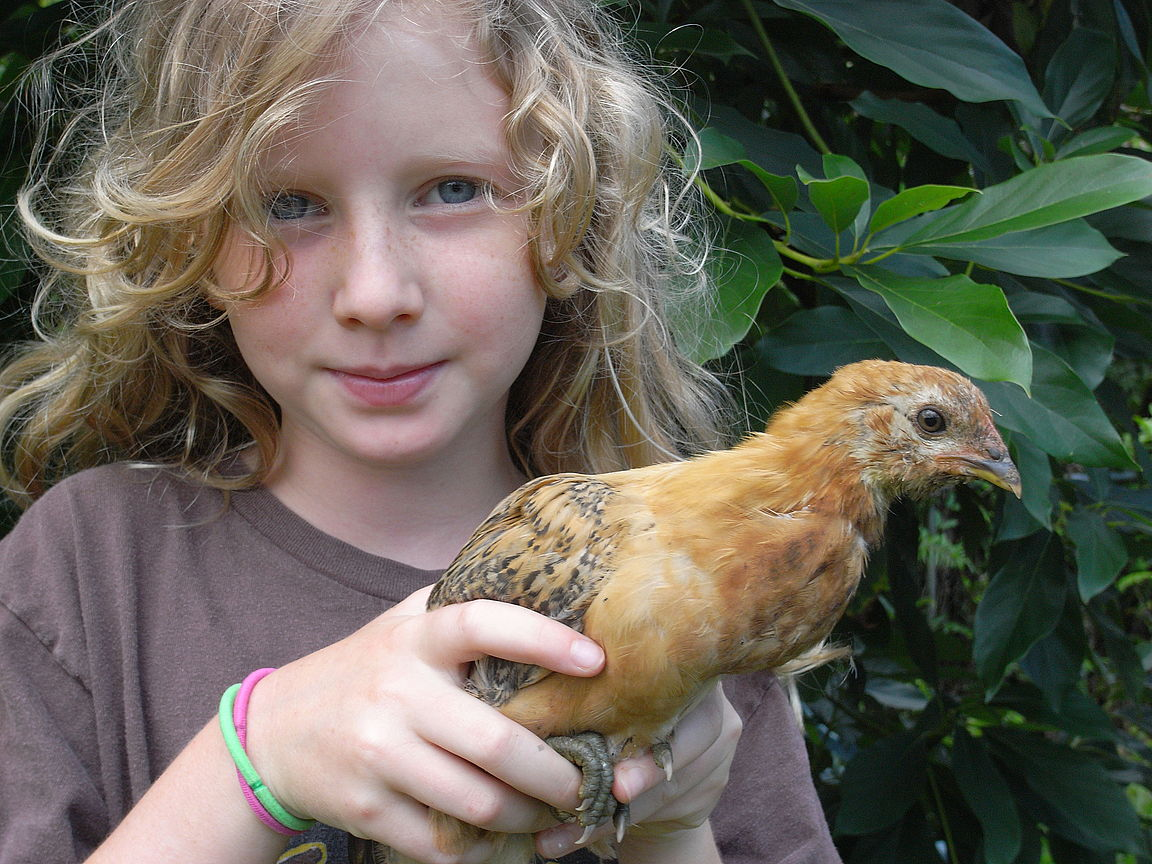
\includegraphics[width=8in]{R20090619-101948}

\begin{center}{\Large ``Harry Potter'' }\end{center}
\newpage

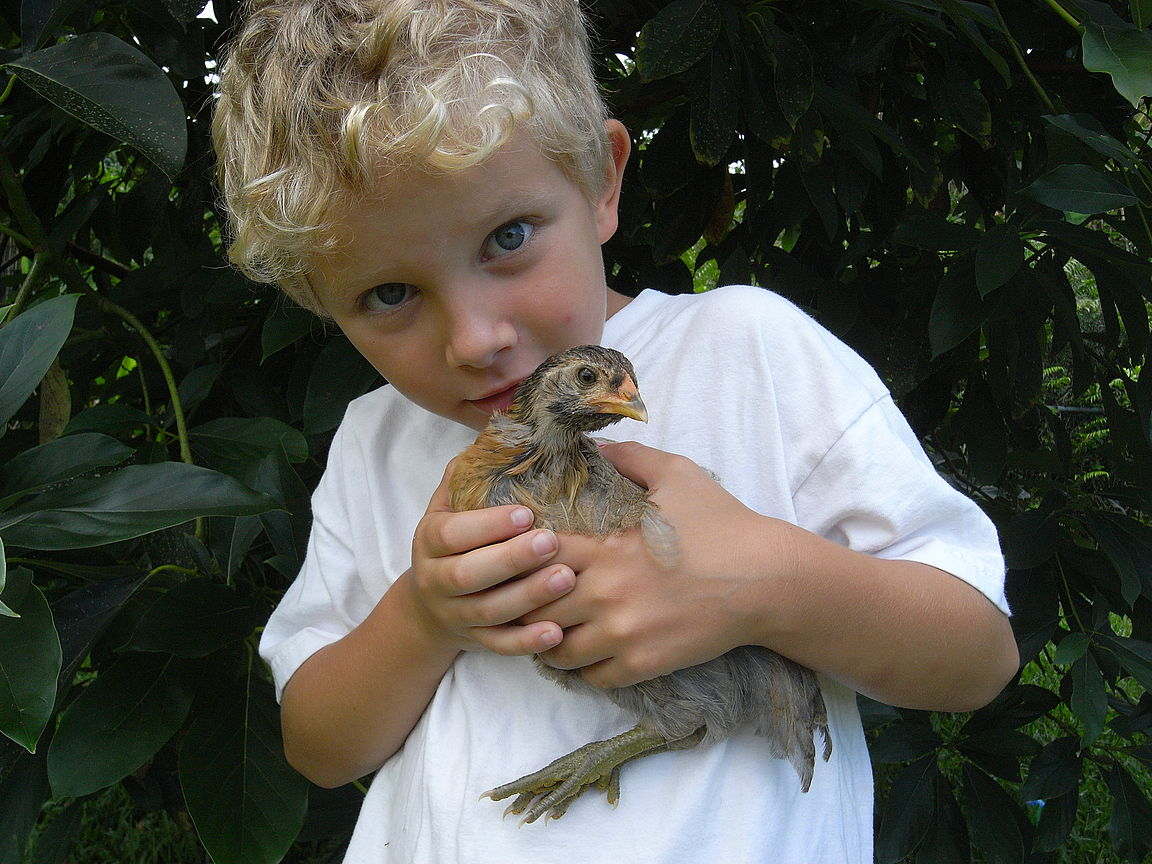
\includegraphics[width=8in]{R20090619-102238}

\begin{center}{\Large ``Junior Junior'' }\end{center}
\newpage

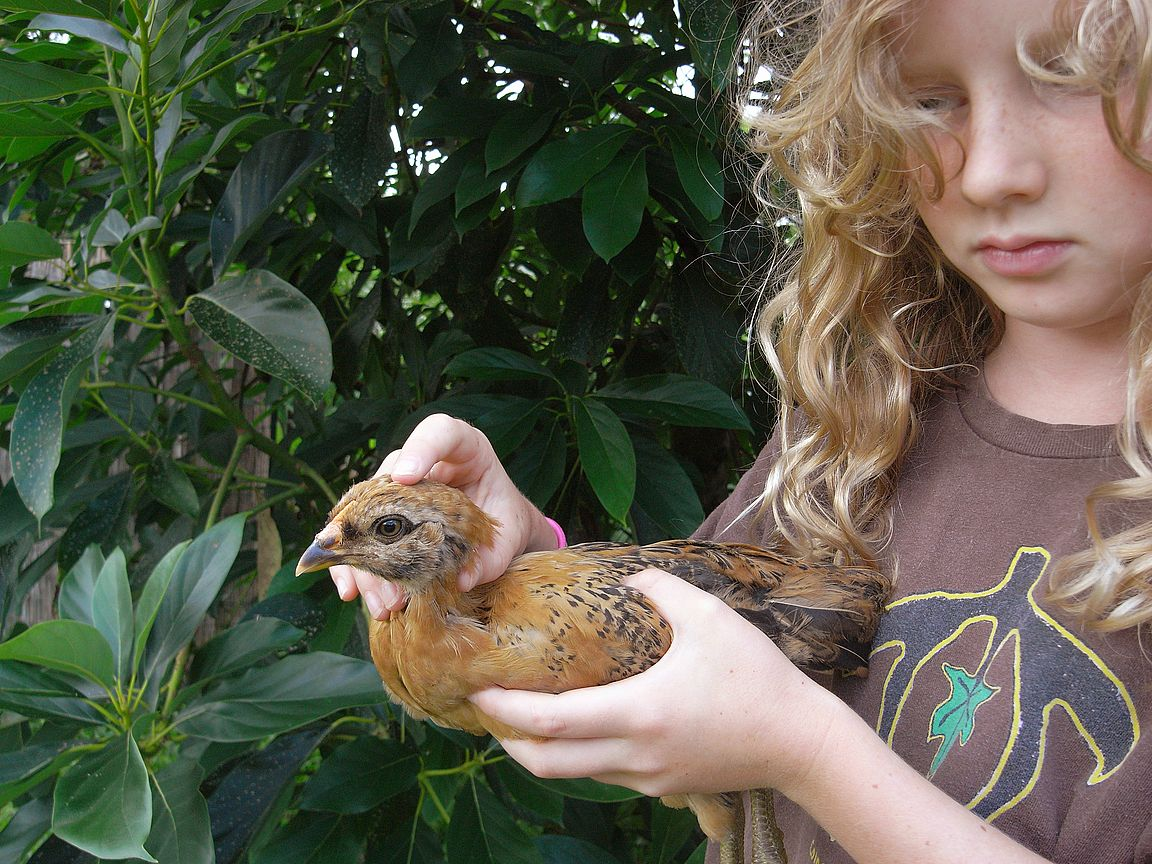
\includegraphics[width=8in]{R20090619-102446-curves}

\begin{center}{\Large ``Ron Weasley'' }\end{center}
\newpage

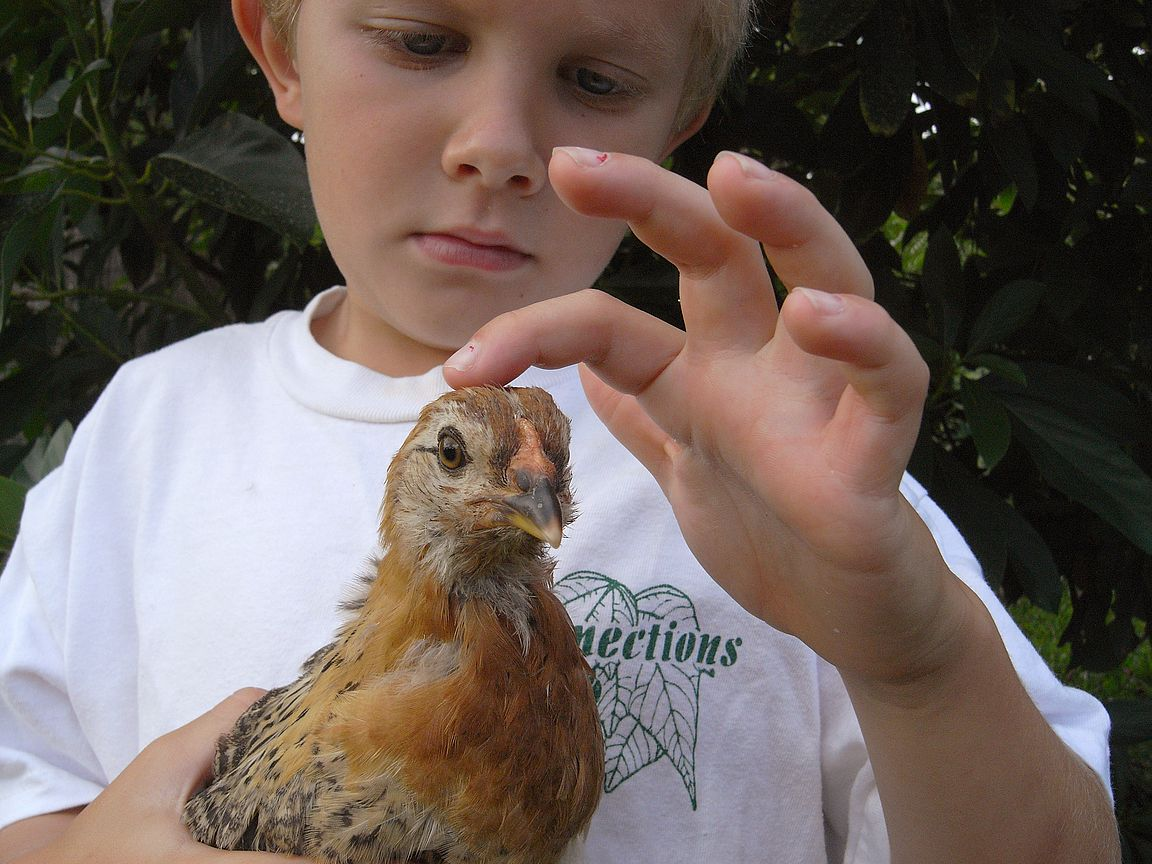
\includegraphics[width=8in]{R20090619-102632-levels}

\begin{center}{\Large ``Junior'' }\end{center}

Yes, there are two Juniors--one is {\em Junior Junior} and the other
is just {\em Junior}. (Don't ask, I didn't name them.) 
\newpage

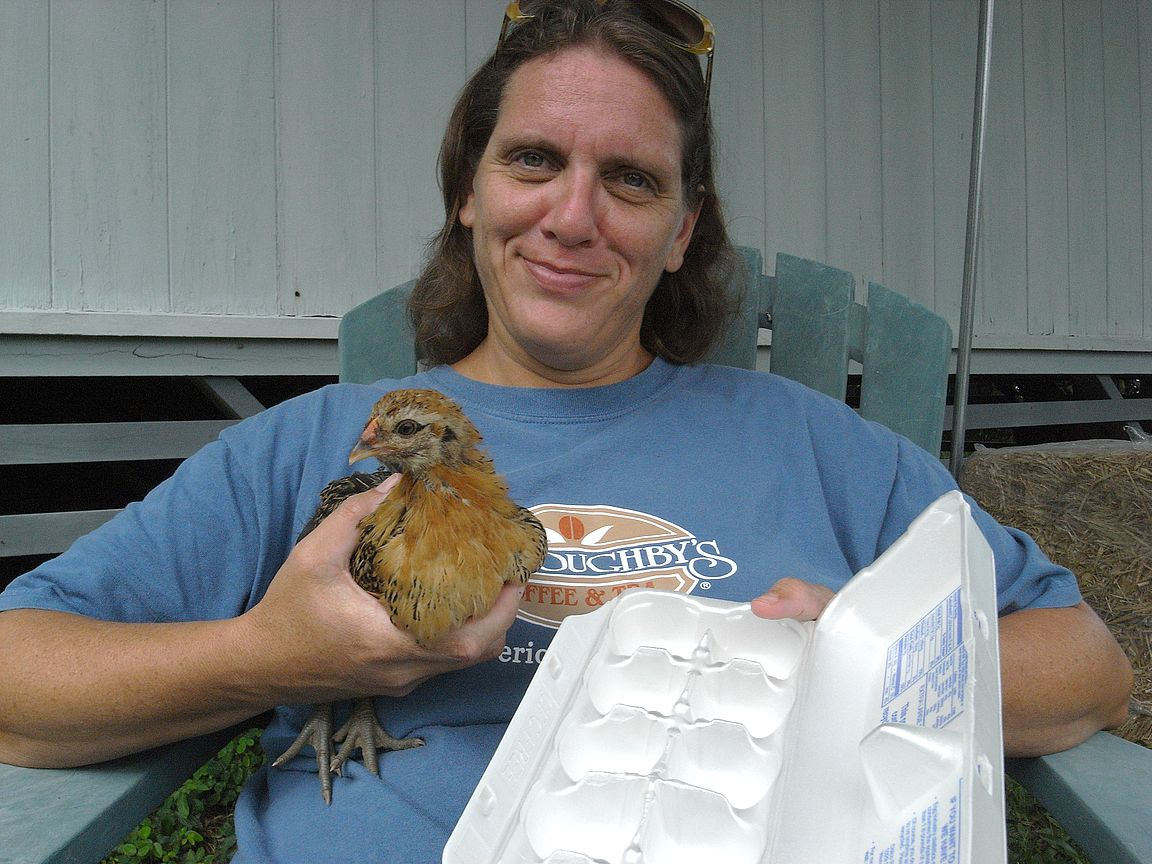
\includegraphics[width=8in]{R20090619-103448-master}

According to everything I've read, they won't start laying until at
least 6 months of age. Suffice it to say I'm looking forward to a
Christmas omlette. 

Ameraucanas lay medium sized eggs that are light green, blue, or
bluish-green. My wife's not so sure about eating green eggs, but I'll
bet one serving of fresh free range eggs will change her mind.
\newpage

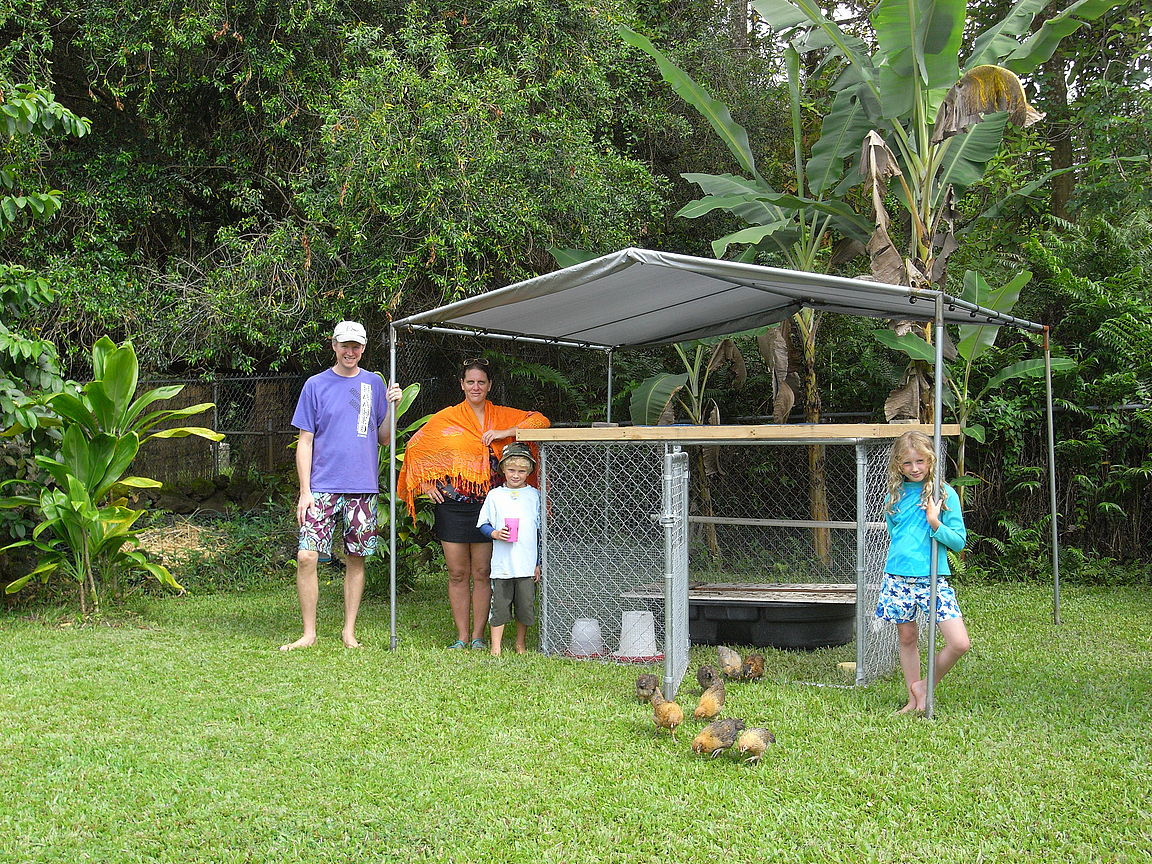
\includegraphics[width=8in]{R20090621-152613}

Back by the bananas, finally, where we wanted the coop originally (see
first photo). The chickens are foraging well and so far Lily hasn't hurt
any, although she does chase them some. Today two got alarmed at the
lawn mower and found a hole in the fence and went into the jungle you
see in the back. Fortunately they quickly made their way back after the
flock moved back to the coop. 

Well, I've run out of time for the book. So we'll say goodbye with a
group shot of the brood. Wish us luck! 
\newpage

\vspace*{1in}

{\LARGE Book Considerations}

Solo Photo Book Month (sofobomo.org) is a DIY project to make a photo
book in one month. All of the photos must be taken and the book laid 
out and processed into a PDF in 31 days. This is my second year
participating in the event, along with many other photographers all over
the world. 
Last year I did square format B\&W, so I was determined to do color and
some sort of rectangular format this year. I chose to go all landscape, 
even though it meant passing on some good verticals I had taken. Also,
last year was more of a series of portraits, and this year I was
determined to have the book tell more of a story. I struggled to find
something that would fit my tight schedule this year when the ``chicken
project'', which I'd had on the back burner, hit me as a good fit to
dovetail with SoFoBoMo. 

If you have a comment to share, thoughts on the book, life with
chickens, technical info, questions, whatever...drop by 

\url{http://redskiesatnight.com/books/chickens-anyone}

and leave a comment. We'd love to hear from you! There you can also
download a PDF version. 

For more information about Solo Photo Book Month, visit

\url{http://sofobomo.org/}

\vspace*{0.25in}

{\LARGE Technical Details}

I was really pressed for time to get the book done in the requisite 30
days this year. I threw it together with snapshots taken with a Ricoh
GX100 camera. No post processing was done except for some quick levels
adjustments in the image editor GIMP.
{\em ImageMagick} was used to batch downsample the images for the web version
(144 dpi) or the book version (300 dpi). 
I designed the book using \LaTeX (with the wonderful {\em xetex} and
{\em xdvipdfmx}) for easier adjustments for dead tree publishing. 
The font used is Garamond. This book was made on Linux.

%END
